%% ----------------------------------------------------------------------
%% START OF FILE
%% ----------------------------------------------------------------------

\documentclass[master,print]{xduthesis}
% \usepackage{showframe}
\usepackage{layout}
\usepackage{listings}  % don't forget [fragile] option after \begin{frame}
\lstset{language=C++, basicstyle=\ttfamily, numbers=none, xleftmargin=5pt, showstringspaces=false, frame=single} %keywordstyle=\color{red}
\usepackage{diagbox}
\usepackage{float}
\usepackage{enumitem}  % 带方括号的列举环境
\usepackage{etoolbox}  % 分支判断用

\newtoggle{blindreview}
\togglefalse{blindreview}
\toggletrue{blindreview} %这行注释打开的话按盲审要求排(隐去作者信息)

\begin{document}
%\layout{}
%%%%%%%%%%%%%%%
%% 论文前置部分
%%%%%%%%%%%%%%%
\frontmatter

% 论文相关信息(封面)
\subjectcode{10701}
\subjectcode{10701}
\iftoggle{blindreview}{
    \studentid{~}
}{
    \studentid{1203121857}
}
\catelognumber{TP311.52}
\secretlevel{公开}

\ctitle{基于SSD的HDD缓存系统研究}
\etitle{A Research of HDD Caching System Based on SSD}

\iftoggle{blindreview}{
    \cauthor{~}
    \eauthor{~}
    \csupervisor{~}
    \esupervisor{~}
}{
\cauthor{闫林}
\eauthor{Yan Lin}
\csupervisor{刘凯~教授}
\esupervisor{Prof. Liu Kai}
}

\cfirstdiscipline{计算机科学与技术}
\efirstdiscipline{Computer Science and Technology}
\cseconddiscipline{计算机应用技术}
\cdegreetype{工程硕士}
\cdate{2014年11月}
\edate{Nov 2014}

% 中英文摘要声明
%% ----------------------------------------------------------------------
%% START OF FILE
%% ----------------------------------------------------------------------

\begin{cabstract}

固态硬盘(SSD)作为一种新兴的存储介质,被应用到存储系统中。固态硬盘较传统硬盘有着许多优势。

\end{cabstract}

\begin{ckeywords}
固态磁盘,混合存储,缓存
\end{ckeywords}

\begin{cthesistype}
应用基础研究类(或基础研究类)
\end{cthesistype}

%% ----------------------------------------------------------------------

\begin{eabstract}

Solid State Disk (SSD), as a new technology, has been introduced into storage subsystem because of its many advantages, such as the compact size, low power consumption and especially the higher performance than Hard Disk Drive (HDD). But due to its relatively high price, currently SSD is mainly used as cache or used in some high-end storage subsystems. Actually, most of times, HDD and SSD exist in a system at the same time, and only used a part of the SSD. If user can use software to configure part of the unused SSD as storage, and another part of the unused SSD as a cache for the HDD, this will improve the IO performance of the whole system.

Using SSD as a cache for HDD not only take performance advantage of SSD and save costs to replace all storage to SSD, but also ensure the storage system reliability. Using the data locality theory, the requested hot data on HDD will be moved to SSD,
Performance : Store hot data on SDD while leaving cold data in disk

Reliability: SSD is non-volatile compared with DRAM

The system is implement as a Windows volume storage filter driver. Run in two mode: SSD as cache with write through and SSD as cache with write back. The results show the SSD cache can bring system with 10x read enhancement with wt and wb.

\end{eabstract}

\begin{ekeywords}
SSD, Hybrid Storage, Cache
\end{ekeywords}

\begin{ethesistype}
Applied Basic Research(or Basic Research)
\end{ethesistype}

%% ----------------------------------------------------------------------
%%% END OF FILE 
%% ----------------------------------------------------------------------

% 生成论文的封面、声明页、中英文摘要
\makecover

% 插图索引
\listoffigures
% 表格索引
\listoftables
% 其他列表
%\chapter*{符号对照表}

\chapter*{缩略语对照表}

\begin{tabular}{lll}
缩略语 & 英文全称 & 中文对照\\
HDD        & Hard Disk Driver & 机械硬盘\\
SSD        & Solid State Driver & 固态硬盘\\
SDRAM      & Synchronous Dynamic Random Access Memory & 同步随机存储器\\
NVRAM      & Non-Volatile Random Access Memory & 非易失随机存储器\\
P/E cycles & Program/Erase Cycles & 写入/擦除次数\\
SLC        & Single Level Cell & 单层式储存颗粒\\
MLC        & Multi Level Cell & 多层式储存颗粒\\
TLC        & Triple Level Cell & 三层式储存颗粒\\
RPM        & Rotation Per Minute & 每分钟转动数\\
WDM        & Windows Driver program Model & Windows驱动程序模型\\
LRU        & Least Recently Used & 最近最不使用算法\\
LFU        & Least Frequently Used & 最近最少使用算法\\
IRP        & IO Request Packet & Windows IO请求数据包\\
\end{tabular}

% 论文目录
\tableofcontents

%%%%%%%%%%%%%%%
%% 论文正文
%%%%%%%%%%%%%%%
\mainmatter

%% ----------------------------------------------------------------------
%% START OF FILE
%% ----------------------------------------------------------------------

\chapter{绪论}
\label{cha:introduction}

\section{研究背景}
\label{sec:background}

日新月异的计算机技术发展,带来了数据存储设备容量和CPU处理能力的大幅度提升。然而,磁盘系统的数据带宽以及I/O吞吐率的增长速度并未跟上CPU的步伐。与之而来的是CPU和传统磁盘系统间愈发加大的速度差距\cite{matthews2008intelturbomem}(图\ref{fig:cpu-disk-diff})。

\begin{figure}[H]
\centering
\includegraphics[width=0.7\linewidth]{./graph/cpu-disk-gap}
\caption{CPU与磁盘速度差异}
\label{fig:cpu-disk-diff}
\end{figure}

云端计算\cite{jimgray2003cloud}是继计算机系统从二十世纪80年代的大型计算机到“客户端-服务器”模式的又一次转变。云端计算的对象,大数据(Big Data),同样获得了存储设备厂商对越来越多的关注。大数据之所以出现,是因为我们生活在一个拥有海量数据的信息社会中,21世纪,人们与数据或信息交互比历史上的任何时期都要活跃。46亿全球移动电话用户中,有20亿人访问互联网,人们在畅游互联网的过程中,会自觉或不自觉的产生日志、访问历史和评论等信息,互联网上流动的交通量已经达到每年667艾字节。除了互联网,数据已经渗透到每一个行业和业务职能领域,并逐渐成为重要的生产因素。2011年5月全球知名咨询公司麦肯锡全球研究院发布了一份题为《大数据:创新、竞争和生产力的下一个新领域》的报告,报告指出了人们对于大数据的运用预示着新一波生产率增长和消费者盈余浪潮的到来。

大数据对存储系统的容量、速度及可靠性提出了非常高的要求,一些高性能的存储设备由此产生。固态硬盘(SSD)作为其中的佼佼者被引入传统的以机械硬盘(HDD)为主的存储系统\cite{morris2003evostorage}。从表\ref{tab:ssd-speed-compare}可以看出,固态硬盘的读写性能远远高于传统的机械硬盘\cite{libo2010cacheforssd},将固态硬盘引入存储系统中,可以大大提高系统的I/O性能。

\begin{table}[H]
\centering
\caption{HDD、DRAM和SSD的读写速度比较}
\begin{tabular}{|c|c|c|c|}
\hline  & Hard Disk & DRAM & SSD \\
\hline Read Access & 8.3ms & 60ns & 85ns \\
\hline Write Access & 9.1ms & 60ns & 4-10ms \\
\hline
\end{tabular}
\label{tab:ssd-speed-compare}
\end{table}

然而固态硬盘的价格仍然昂贵,虽然过去几年固态硬盘的价格一直快速下降,但下跌趋势正日益放缓\cite{henry2014ssdprice},一系列问题导致固态硬盘和机械硬盘之间的价格差距不可能会很快消失。因此,固态硬盘不会在短时间内取代机械硬盘成为企业的主要储存设备。

固态硬盘的价格从2005年和2006年的3美元/GB跌至了2012年的0.67美元/GB,但与HDD的0.09美元/GB相比仍然相去甚远。根据固态硬盘历史价格的下降速度计算,到2020年它的价格约为0.15美元/GB,而届时机械硬盘的价格将会降至0.03美元/GB,对存储厂商来说机械硬盘仍然存在难以抗拒的价格优势。

综上所述,鉴于固态硬盘的价格较高且存储密度与机械硬盘差距较大,目前来讲,完全使用固态硬盘替代机械硬盘作为存储设备的条件还不够成熟。虽然已有一些云计算存储中心部署了全固态硬盘的存储阵列,但是过高的成本令大多数使用者望而却步。为此,本文设计了一种既能保证成本在可接受的范围内,又能充分利用固态硬盘高I|/O性能的混合存储解决方案。

\section{相关研究工作}
\label{sec:related_works}

针对固态硬盘价格高、功耗低、容量小、读写性能高等特点,很多公司和研究者针对固态硬盘的使用场景,提出了一些基于固态硬盘的混合存储或分级存储的解决方案。这些方案与全固态硬盘解决方案从价格上更能被接受。同时,相比于传统的使用DRAM作为缓冲,固态硬盘有着非易失性、功耗低(表\ref{tab:ssd-power-compare})\cite{taeho2006flashcache}、存储密度高、可扩展性强的优势。

\begin{table}[H]
\centering
\caption{DRAM、Flash功耗比较}
\begin{tabular}{|c|c|c|c|}
\hline
\diagbox{介质}{功耗} & Density-Gb/cm2 & Active Power* & Idel Power* \\
\hline DDR2 DRAM & 0.7 & 878mW & 80mW \\
\hline NOR & 0.75 & 86mW & 16μW \\
\hline NAND & 1.42 & 28mW & 6μW \\
\hline
\end{tabular}
\\ * Power consumed for 1Gbit of memory
\label{tab:ssd-power-compare}
\end{table}

全球第六大企业软件公司EMC在2012年推出了VFCache解决方案\cite{vfcache}。该解决方案将EMC VFCache智能缓存软件与LSI的第二代PCIe闪存适配器系列LSI Nytro WarpDrive卡相结合,进一步加速应用性能,改善了EMC存储环境下Cisco服务器的响应时间。VFCache通过拦截不超过64KB大小的读写请求(通常为随机操作)并将其缓存到PCIe闪存卡,达到加速访问的效果。由于不缓存应用程序的写操作,而是直接通过FCHBA卡写入后端SAN存储并等待其反馈成功信息,因此,即使VFCache出现硬件故障也不会导致数据丢失。通过将固态硬盘引进存储阵列,EMC成为第一家涉足服务器PCIe闪存市场的主流厂商。

华为的云计算存储部门提出了SmartCache解决方案\cite{smartcache}。SmartCache是一种将固态硬盘作为缓存资源的分层存储技术,是华为服务器集群使用的一个动态数据缓存解决方案。SmartCache通过充当内存的扩展的方式,显著降低延迟并加快随机IO敏感性应用程序的执行速度,而无需以物理方式将数据移动到固态硬盘上。使用一个或多个固态硬盘作为磁盘阵列的缓存,称为SmartCache缓存池。通过统计HDD访问的热点数据,每隔一段时间移动数据到SSD的缓存池中。当热数据被访问时,就可以直接从缓存池中读取。该方案主要适用于IO请求中大部分为读,存在热点数据区域,且位置随机的小块请求的场景。

LSI作为一家知名的生产RAID适配器的公司,针对混合存储的市场需求,也专门推出了型号为LSI MegaRAID的SATA+SAS RAID控制卡。该RAID卡的特点在于,采用固态硬盘作为磁盘阵列的缓存存储热数据,从而有效提高读写性能,降低I/O时延,缩短RAID的访问和重建时间。结合LSI MegaRAID CacheCade Pro2.0软件\cite{lsiraidcache},可以动态地将热数据从HDD阵列到SSD高速缓存中,操作完全透明,无需进行手动配置。

FC/SAS企业级闪存驱动器制造商STEC开源了自主研发的Linux系统下的EnhanceIO混合存储软件\cite{enhanceio},EnhanceIO能够加速任意类型的块存储设备——DAS/RAID/iSCSI/FC SAN。此外,EnhanceIO可以支持任意品牌型号的固态硬盘(包括SAS、SATA、PCIe和 Fibre Channel)作为缓存,同时针对STEC的产品有优化。缓存策略方面,EnhanceIO具备Read Cache(读缓存)、Write Back Cache(写回)和Write-through Cache(写通)三种模式,并能够在异常断电时保证用户数据不会丢失。

另一家SSD生产厂商,STEC的竞争对手Fusion-io也提出了自己的固态硬盘混合存储解决方案Fusion-io ioControl Hybrid Storage Solution\cite{fusionio}。与STEC不同的是,该解决方案针对云计算,能够很好的与虚拟机平台VMware Workstation以及Microsoft SQL Server Clusters整合在一起,提高虚拟机运行速度和减少数据库查询的响应延迟。

\section{全文组织结构}
\label{sec:organization}

为提升混合存储系统性能,本文提出并实现了一种使用固态硬盘作为传统机械硬盘缓存的解决方案。该方案能够在保证系统正确性和稳定性的前提下,提升存储系统的I/O性能。

论文的全文组织结构如下。

第一章:绪论。论述当前云计算和大数据处理背景下对于存储系统的性能需求,固态硬盘和机械硬盘混合存储系统的存在现状。简要描述论文的研究意义以及国内外的相关研究工作。

第二章:相关技术简介。介绍与论文关系紧密的相关软硬件技术,包括固态硬盘的原理和特性、缓存系统的发展和评估、混合存储系统的原理和分类。

第三章:关键技术。详细介绍实现论文提出解决方案实现过程中所涉及的关键技术,包括磁盘IO的捕获方式、缓存系统使用的页面替换算法、缓存空间的映射策略和缓存块使用的索引结构以及缓存系统提供的两种回写策略。

第四章:缓存系统的具体实现。描述论文抽象出的缓存页面替换算法的公共接口,并对每个接口的具体实现细节加以介绍。介绍磁盘IO捕获函数的实现逻辑。用户配置工具提供的配置参数,以及缓存系统的其他实现细节。

第五章:实验和结果分析。从稳定性和性能两个角度对实现的系统进行测试,分析测试结果。与商业缓存软件进行比较,对比缓存系统对机械硬盘的性能提升比例。

第六章:总结与展望。总结论文的研究成果和解决方案的贡献,展望进一步提升系统性能的可行方案。

%% ----------------------------------------------------------------------
%%% END OF FILE
%% ----------------------------------------------------------------------
%% ----------------------------------------------------------------------
%% START OF FILE
%% ----------------------------------------------------------------------

\chapter{相关技术简介}
\label{cha:related_work}

\section{存储介质简介}

\subsection{机械硬盘(HDD)}
机械硬盘\cite{hdd2009}(HDD,Hard Disk Driver)是个人计算机中一种应用最为广泛的非易失性的存储设备,使用覆盖有氧化铁的坚硬旋转盘片为存储介质。机械硬盘内部的物理结构分为磁盘、电动机、悬臂和主控芯片几部分。磁盘盘面以磁道、柱面和扇区的方式组织表面空间。由电动机带动盘片旋转,副电动机带动悬臂上的磁头移动到碟片表面的某个位置。磁头悬浮在磁盘的正反两面上,磁盘旋转时磁头会在盘片表画出一个与磁盘同心的圆形轨道(称磁道或柱面)。此时,磁头内部的磁感线圈感应磁盘上的磁铁极性,通过时间间隔定位扇区,通过电流读取、写入数据内容到当前磁头所处的扇区。

通过磁化盘片表面上磁铁单元的极性,机械硬盘在平整的磁性表面上存储最基础的01比特数据。离磁性表面很近的读写磁头利用磁铁单元对电流的电感效应完成读写。盘片的两个存储面上各存在一个磁头负责读写,所有磁头的水平运用方向保持一致,磁头的移动方向由磁头控制器所负责。磁头只能沿盘片半径在水平方向上运动,结合电机带动盘片的高速旋转,磁头可以定位到盘片正反面上的任意位置进行记录数据的读写操作。

\begin{figure}[H]
\centering
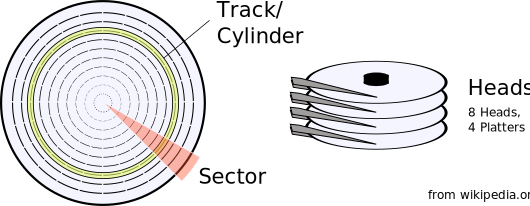
\includegraphics[width=0.6\linewidth]{./graph/hdd-struct}
\caption{机械硬盘结构}
\label{fig:hdd-struct}
\end{figure}

\begin{itemize}
\item 磁道
\\当磁头保持在某个位置上时,磁盘旋转,磁头会在磁盘表面画出一个与磁盘同心的圆圈,我们称圆圈的轨迹叫做磁道(Track)。
\item 柱面
\\磁盘中通常存在一或多个盘片,竖直上的不同盘片、水平上处于同一半径的多个圆形磁道组成的一个圆柱面(Cylinder)。
\item 扇区
\\每个圆形磁道按照角度又被等分为若干个弧段,每个弧段是硬盘上的一个扇区(Sector)。一般称磁盘的首个扇区为引导扇区。
\end{itemize}

一般以RPM(每分钟的转动数)为单位描述机械硬盘盘片旋转速度,存在5400、7200、10000、15000几种规格。电机带动盘片转速越高,数据读写速率愈快,但噪音和发热量也上升明显。7200转属于最常见的磁盘转速。

机械硬盘内部的盘片、磁头机械结构决定了机械硬盘擅长于顺序读写,随机读写性能较差。

\subsection{固态硬盘(SSD)}
固态硬盘\cite{ssd2009}(SSD,Solid State Driver)作为一种存储设备,既可以基于永久性存储介质,如Flash闪存,也可以基于非永久性存储介质,如同步动态随机存取存储器(SDRAM)。设计固态硬盘的初衷是为了替代传统机械硬盘。固态硬盘内部已没有了像机械硬盘那样可以旋转的盘片结构,但是为了兼容人们对存储设备的命名习惯,固态存储器仍被称作硬盘。根据上面提到的所基于的两种存储介质,固态硬盘分为易失性和非易失性两类。

\begin{enumerate}
\item 基于易失性记忆体的固态硬盘

使用易失性记忆体作为存储介质的固态硬盘,通常用于临时存放数据。易失性记忆体需要外界电力维持其内部的记忆功能,因此为了防止断电时的数据丢失,一般需要配合电池进行不间断供电。以SDRAM为代表的易失性存储介质,具有访问速度快(接近内存速度)、使用寿命长的优点。利用速度上的优点,软件程序可将需要访问的数据从机械硬盘转存到固态硬盘中,以此减少机械硬盘电机的启停延迟、磁头的寻道延迟对数据访问速度的影响。

此外,基于易失性记忆体的固态硬盘还可用于应急备份。这类固态硬盘一般会使用电池提供备用电力,即使遭遇意外停电,固态硬盘还可短暂利用电池电力,将数据转移到非易失存储设备。恢复电力后,再将数据从非易失存储设备转移过来。

\item 基于非易失性记忆体的固态硬盘

基于非易失性记忆体的固态硬盘在外观上和机械硬盘已经没有什么区别。以NVRAM为代表的非易失性存储介质的数据存取速度,介于易失性介质SDRAM和机械硬盘之间。相比于易失性介质,非易失性介质数据一经写入,便无需额外电力以维持其存储能力,不必考虑断电的影响使其更有潜力替代常规硬盘。

每块固态硬盘内部都会存在多个存储颗粒,每个存储颗粒中有非常多的存储单元储存数据。目前,市面上存在三种主流的制造固态硬盘存储单元的NVRAM颗粒,分別是多层式储存颗粒(MLC,Multi Level Cell)、单层式储存颗粒(SLC,Single Level Cell)和三层式储存颗粒(TLC,Triple Level Cell)。SLC、MLC和TLC三者的区别是存储颗粒内部单个存储单元所能存储的状态个数:SLC一种,MLC两种,TLC三种。这三者的读写速度几乎没有差别。TLC颗粒主要在企业级固态硬盘中使用,但是成本很高,使用MLC和TLC颗粒制造的固态硬盘的成本低,但是寿命较短。

由于存储颗粒内部每个存储单元的写入次数是有限的,存储颗粒的最大写入次数便是存储颗粒的使用寿命。固态硬盘控制器通常会把写操作平均分配到存储颗粒内部的每个存储单元上,再通过映射表的方式定位数据的实际存储位置。工业界使用P/E cycle这一参数标准衡量固态硬盘的使用寿命,一个P/E cycle代表了固态硬盘内所有的存储颗粒被写入一次。固态硬盘的P/E cycle参数体现了硬盘内部存储颗粒可写入次数的峰值,P/E cycle越大固态硬盘的使用寿命越长。

\begin{table}[htb]
\centering
\caption{SLC、MLC和TLC的寿命和价格比较}
\begin{tabular}{|c|c|c|c|}
\hline  & SLC NAND Flash & MLC NAND Flash & TLC NAND Flash \\
\hline P/E Cycles & 100,000 & 10,000 & 4,000 \\
\hline Cell type & 1bit/cell & 2bit/cell & 3bit/cell \\
\hline Price (USD/GB) & 5 & 1.4 & 1 \\
\hline
\end{tabular}
\label{tab:slc-mlc-tlc-compare}
\end{table}

从表\ref{tab:slc-mlc-tlc-compare}可以看出,存储颗的粒密度从SLC到TLC逐渐增大,而P/E cycle逐渐减少。SLC颗粒常被用于生产企业级的固态硬盘,而MLC颗粒和TLC颗粒则较多的出现于桌面计算机的固态硬盘中。虽然TLC颗粒的P/E cycle与SLC颗粒存在将近两个数量级的差距,但实际应用情况表明,使用TLC存储颗粒的固态硬盘完全可以满足桌面计算机的使用寿命要求。

尽管相比较于机械硬盘,固态硬盘有着如此多的优势,但使用非易失性颗粒的固态硬盘并不是不存在缺点。在硬盘剩余空闲空间不多时,极有可能出现严重影响写入性能的Write cliff现象。Write cliff现象出现在当所有存储颗粒的空闲页都已经被初始化写入,新的写请求无法一次性得到足够的空闲页以完成写入操作的情况下。此时,固态硬盘控制器必须要擦除某些未写满的存储页面再进行写操作:控制器会将未写满存储页面的原有数据拷贝到临时空间,再进擦除;将原有数据与新数据进行合并,写入到擦除后的存储页面。拷贝原有数据到临时空间消耗的时间是Write cliff出现的主要原因。

固态硬盘厂商为了减少Write cliff对性能的影响,特别加入了特别针对固态硬盘删除数据的TRIM指令。当需要删除文件时,可通过TRIM指令会告知固态硬盘被删除文件的位置,固态硬盘控制器会将对应的存储块标记为空闲状态。这样,就能在一定程度上保证总是存在空闲页,从而降低Write cliff现象出现的概率。TRIM指令的出现,很大程度上提升了固态硬盘的性能、延长了固态硬盘的寿命,但当空闲页面无法满足写请求时,仍然需要擦除未写满的存储页面。可以得出的结论是,TRIM命令只能推迟而无法避免Write cliff现象的出现。
\end{enumerate}

\subsection{机械硬盘与固态硬盘的比较}
固态硬盘出现的目的是替代传统的机械硬盘,但是机械硬盘相较于固态硬盘的某些优势使得固态硬盘不可能在短期内动摇机械硬盘的统治地位。两者之间的差距可从以下几个方面进行比较。

\begin{enumerate}
\item 安全性
\\机械硬盘内部的盘片、电机等机械构造决定了在发生碰撞和震动时,磁头和盘片的接触往往会造成机械硬盘的损坏,从而导致数据的丢失。固态硬盘内部使用的缓存芯片几乎不受碰撞和震动的物理影响。
\item 性能
\\无论是启动速度还是IO性能,固态硬盘都有着非常明显的优势。造成这种优势的主要原因是固态硬盘内部不是机械结构,不需要寻道以定位数据。传统的机械硬盘则需要在指令接受后开始寻道。因此固态硬盘在读写速度,尤其是随机读写上,较普通机械硬盘存在很大优势。
\item 价格
\\2012年的统计数据表明,固态硬盘的价格是0.67美元/GB,传统的机械硬盘的价格是0.09美元/GB,固态硬盘价格是机械硬盘的7倍多。造成价格悬殊的主要因素是机械硬盘发展较早,技术相对成熟;固态硬盘制造工艺则有待提高。固态硬盘的高昂价格会让很多用户在购买前三思,他们更倾向于暂失固态硬盘的诸多优势而选择性价比更高的机械硬盘。
\item 容量
\\海量数据时代的到来和用户对更高品质交互体验的追求,带来了日益增长的数据存储空间需求。大容量固态硬盘不仅非常稀少且价格昂贵,主流的固态硬盘一般都为128GB、256GB或512GB的存储空间。实际情况是,1TB的机械硬盘都已难以满足桌面电脑的需求,更不用说数据量巨大的企业级用户。
\item 耗电量
\\机械硬盘使用电机驱动盘片旋转和磁头移动,耗电量约为固态硬盘的3倍多。对于移动设备来讲,耗电量的多少是衡量电池所能支持待机时间的关键。同样的,在存在上百个磁盘阵列的数据中心部署固态硬盘,可以节约大量电能,从而减少电费支出。但基于易失性存储器的固态硬盘需要不间断供电,否则可能会导致数据丢失。
\item 重量和形状
\\由于不存在机械硬件的磁盘、电机等部件,固态硬盘的平均重量仅仅有70-85克,而机械硬盘则可达到650-800克,这一优势可使便携的移动设备同时搭载几个固态硬盘成为可能。同时,完全半导体化的固态硬盘内部结构,使其在物理上无样式、结构的限制,可根据实际需求改变固态硬盘的接口、形状。
\item 工作温度
\\由于固态硬盘本身的功耗就不高,所以其在工作过程中产热也相对较低。而机械硬盘每分钟5000转以上的转速,盘片和空气的摩擦以及不同机械部件之间的摩擦所产生的热量远高于固态硬盘,温度太高很容易使机械硬盘的脱离正常工作状态。固态硬盘不但本身产生的热量少,而且能够工作在更宽泛的温度范围内。
\item 噪音
\\ 得益于使用闪存芯片不存在机械构件,固态硬盘不会产生噪音。而机械硬盘运行时则会产生一定的噪音。尤其是存储中心大规模的磁盘阵列所产生的巨大噪音,更是需要设立专门的机房进行存放。
\end{enumerate}

\section{存储系统缓存技术}
\label{sec:storage_cache_tech}

尽管自二十世纪九十年代以来,计算机硬件技术的发展带来了磁盘存储密度每半年到一年一倍的提升,但没有相应的技术能够以同样的速度缩短存储介质的访问时间。缓存技术\cite{cache2011}作为一种减少IO子系统的响应时间、增加系统吞吐量的解决方案,已被广泛应用于存储子系统中。

\subsection{缓存的特点}
保存了主存储器中少部分数据复制品的缓存,其访问速度远高于主存储器。如果使用缓存中的数据就可以满足某个访问主存储器的请求,则称缓存命中了一次。

由于缓存中保存的是主存储器中的部分数据,因此会出现找不到所需数据而无法命中的情况,此时则需要访问主存储器才能获得数据。如果这种情况发生的比例超过一定数值,缓存对系统性能的提升就无法得到保证。不命中情况下获得的主存储器数据被用来更新缓存内的数据内容,以便下次访问不再需要到主存储器中获取数据。由于被频繁访问的数据并不是一成不变的,因此需要缓存页面替换算法不定期的更新缓存内的数据,这样才能保证缓存中的数据是被访问最频繁的,命中率才有保证。

\subsection{缓存的工作原理}
为了形象说明缓存系统的工作原理,本小节会以CPU访问内存中的数据为例进行说明。绝大多数CPU中都集成了一或多级的高速缓存以缩短访问内存的时间。

CPU执行过程中需要内存中的某个数据时,首先会从高速缓存中查找,如果能够找到,则无需访问内存CPU即可进行处理,几乎没相应延迟;如果没有找到,就只能从响应延迟高的内存中读取后传送给CPU进行处理,同时,将获得的数据块调入高速缓存中。更新缓存中的数据一定程度上可以增加数据在缓存中进行的概率,减少内存的访问。正是这一机制使大多数CPU可达到90\%左右的高速缓存命中率,只有10\%的访问操作需要真正读取内存。减少了需要CPU直接访问内存的次数,也就使得CPU几乎无需等待,就能获得所需数据。一般来说,CPU需要数据时总是先查缓存、后访内存。

\subsection{缓存数据替换算法}
缓存系统运行过程中,需要对存储设备上的数据按照请求的频率进行冷热程度的划分。性能较高的存储设备储存经常访问的热数据,存储在性能较低的设备储存不经常访问的冷数据,以达到区分对待冷热数据的效果。缓存数据替换算法在缓存系统运行过程中,通过识别出的冷热数据,不断移动和更新缓存中数据,尽可能保证热数据存储在性能较高的存储设备,以达到提升缓存命中率和系统性能的目的。所以,从本质上讲,缓存数据替换算法就是数据的热度识别和存储组织管理算法。

从缓存提升系统性能的原理不难得出,区分冷热数据的准确程度直接影响了缓存系统的IO性能。学术上已经有很多关于区分冷热数据的算法研究成果。根据缓存空间组织的粒度,缓存数据替换算法可以分为两类,不同类型算法的识别的准确程度和计算复杂度会有不同。下面将逐一进行介绍。

\begin{enumerate}
\item 数据块级

数据块是最小的数据空间划分单位,通过数据块识别冷热数据需要将主存储空间和缓存空间按照相同大小的数据块进行划分。将数据块看作是统计冷热程度的最小单位,通过统计每个数据块的访问计数,将标记访问计数大的数据块为热数据块。固态硬盘内部的设计中,数据块的热点识别还可用于固态硬盘的损耗平衡:通过一定的映射策略,将写操作平均分配到所有的存储块。

数据块级的冷热数据识别的优势在于,它可以在文件系统无关的存储层面精确地定位出所有的热数据块,同时又不必在考虑例如存储空间组织结构、文件系统等宏观的信息,从而简化了识别冷热数据的计算过程,保证了系统性能受计算复杂度的影响尽可能小。

\item 文件级

文件级别的冷热数据划分\cite{linlin2011}是另一种缓存数据替换算法用到的判定方法。这种以文件作为热度统计的最小单位的方法,为每个文件开辟专门用于保存访问计数的元数据区域。所有的文件访问操作都会对改变元数据区域中的访问计数值。文件级别的冷热数据划分可以从文件类型、文件大小、同时打开文件的进程数目等多种宏观层面指标进行综合判别,提升判别的准确程度。

相比于数据块级别,文件级的判定更能够节省统计数据的存储空间,进而减少缓存系统额外的缓存空间消耗。而且还可以将随机性因素加入文件访问的识别过程,更好的区分冷热数据文件。
\end{enumerate}

\subsection{缓存系统存在的目的}
缓存系统的存在通常是为了达到三个目标:
\begin{itemize}
\item 减少交互的通讯量:缓存数据能最小化在进程和网络间传输的数据量。
\item 降低系统中的处理量:记录处理结果,避免数据的重复处理。
\item 降低主存储器的访问次数:如操作系统内核在内存中缓存的机械硬盘数据。
\end{itemize}

在评估一个缓存系统的好坏时,一般会从性能、稳定性和可用性三个方面进行:
\begin{itemize}
\item 性能:定量分析访存请求在缓存中的命中率和带来的延迟的缩短。
\item 稳定性:缓存算法本身是否稳定性,对于意外情况(如掉电),能否保证数据完整。
\item 可用性:缓存系统对应用是透明的,应用感受到的,仅仅是飞快的响应速度和良好的可用性。
\end{itemize}

\section{混合存储系统}
\label{sec:hybrid_storage}

只要数据的处理速度和存储介质的访问速度、不同类型存储介质的访问速度仍然保持较大的差距,学术界和工业界就不会停止研究和探索利用不同速度的存储器件,搭建混合存储系统\cite{zhuqing2013hybrid}以提高系统的性能、容量和可靠性等指标。通过近二十年的研究,科学家和工程师们已经获得了众多的研究成果。

\subsection{基于DRAM与机械硬盘的混合存储}

使用DRAM为机械硬盘缓存数据\cite{sdramcache2002},毫无疑问,是提高机械硬盘性能的重要手段之一。几乎所有操作系统在设计磁盘驱动程序时,都会优先考虑使用DRAM缓存机械硬盘的数据。硬盘制造商在制造硬盘时,同样会在硬盘控制器中加入8-16MB的DRAM芯片。利用数据的空间局部性原理,硬盘控制器在处理IO请求时读取的数据量会略大于请求的数据量,并在DRAM进行缓存。处于硬盘控制器中的DRAM缓存对于软件来说是透明的,磁盘驱动程序不必关心控制器缓存的运行情况。

由于DRAM的易失性限制,通常只用使用DRAM作为读缓存提高机械硬盘的性能,对写性能几乎起不到提高的效果。如果也缓存写操作,为了避免写入机械硬盘的脏数据由于掉电而丢失,磁盘控制器或是驱动程序就必须将脏数据持续的从DRAM写回到机械硬盘,以降低数据丢失的风险。因此,使用DRAM缓存面临着数据可靠性和读写性能间的两难选择,缓存越大性能提升越明显,停留在缓存中的脏数据丢失的可能性也就越大。基于以上原因的考虑,任何缓存系统都会限制缓存中脏数据的停留时间和所占比例。

\subsection{基于NVRAM与机械硬盘的混合存储}

NVRAM存储数据非易失性的优势,使得利用NVRAM缓存提升存储系统写性能成为可能。常用的一种策略是整合NVRAM缓存与DRAM缓存\cite{nvramcache2013},遇到写操作时,同步写入数据到两种缓存。NVRAM的非易失性保证了数据的可靠性,DRAM的高性能保证了性能的提升比例,只有意外掉电时,NVRAM内的备份数据才会被启用,并重新写回到机械硬盘;另一种策略是组合DRAM和NVRAM为一个单一的存储空间,缓存块存储于哪种类型的存储器由算法觉得,但写操作的脏数据块必须存放在于NVRAM中。

NVRAM的小容量特性,使得其对机械硬盘性能提升的贡献非常有限。虽然近5年来的技术革新带来了NVRAM容量的不断提高,但是相比于增长更为迅速的机械硬盘存储空间,加上海量数据访问时通常呈现出的一次访问的特征,使得基于NVRAM与机械硬盘的混合存储的缓存命中率难以有大的提升,对于系统读写性能的提升效果非常有限。

\subsection{高低转速磁盘的混合存储}

机械硬盘中磁盘盘片的物理转速直接决定了读写请求处理的速度。因此,混合不同接口、不同转速的机械硬盘构成设计混合存储系统,曾一度是20世纪90年代存储界研究的热点之一。

高低转速磁盘混合存储的原理是:根据数据的访问热度、保留时间、优先级等指标,将访问频繁的热数据存储在转速为10000-15000 RPM的高性能SCSI机械硬盘中;访问热度低的冷数据则被存储在转速为5400-7200 RPM的性能普通的IDE或SATA机械硬盘中。但由于机械硬盘内部物理器件极限的限制,机械硬盘的不同转速所带来的性能差距并不显著。因此,这种混存系统近些年来已很少被使用。

\subsection{基于固态硬盘和机械硬盘的混合存储}

固态硬盘和机械硬盘之间性能的良好互补性,以及近几年来高寿命、高密度的固态硬盘存储设备生产技术的日渐成熟,这些都为设计基于固态硬盘和机械硬盘的混合存储系统提供了崭新的契机。这种混合存储解决方案已成为海量数据存储技术中的一个新的发展方向,并已经成为了学术界的研究热点。理论研究的发展同时带来了企业存储解决方案如雨后春笋般的提出。Microsoft,LSI,Intel,EMC,IBM, FusionIO等企业都已经或即将推出基于固态硬盘的混合存储解决方案。

\section{缓存算法评估}
\label{sec:cache_evaluation}

大多数学术论文在评估某种缓存替换算法的优劣时,都是只评估替换算法带来的缓存命中率。为了提高论文的说服力,有的还会给出该算法应用于某种环境所带来的性能提升比例。当工程师为混存系统挑选一种合适的缓存算法时,这些数据的参考价值都很有限,且不存在一种通用的评估方法。
下面介绍一种本论文提出并使用的缓存算法的评估模型,该模型既可以用于评估缓存算法给系统可能带来的性能提升,又可以为缓存系统工程师设计系统起到指导作用。

给出评估方法之前,式\ref{equ:cache_evaluation_syms}列出了推理中用到的数学符号。
\begin{equation}
\begin{split}
\\&T_1=\mbox{无缓存时,单个读/写请求处理时间}
\\&T_2=\mbox{有缓存且缓存命中时,单个读/写请求的处理时间}
\\&T_3=\mbox{有缓存但缓存时,单个读/写请求的处理时间}
\\&N=\mbox{读写请求总数量}
\\&R=\mbox{缓存命中率},R\in\lbrack0,1)
\\&T_q=\mbox{查询一个读/写请求在缓存池中是否命中的时长}
\\&T_c=\mbox{从缓存池拷贝或向缓存池写入完成一个读/写请求所需数据的时长}
\\&T_u=\mbox{使用单个未命中的读/写请求数据,更新缓存池所需时间}
\end{split}
\label{equ:cache_evaluation_syms}
\end{equation}

评估缓存对于系统IO性能的提升,可以用有、无缓存前提下,读写请求花费总时长的变化比例来表示。

\begin{equation}
\begin{split}
\mbox{性能提升比例}&=\frac{\mbox{无缓存条件下完成所有读写请求的总时长}}{\mbox{存在缓存时完成所有读写请求的总时长}}
\\&=\frac{NT_1}{NRT_2+N(1-R)T_3}
\\&=\frac{T_1}{RT_2+T_3-RT_3}
\\&=\frac{T_1}{T_3-(T_3-T_2)R}
\end{split}
\label{equ:cache_evaluation_enhance1}
\end{equation}

系统不存在缓存时,一个读/写请求所需的时间($T_1$)等同于该读/写请求直接应用于存储介质上所需的时间。

系统存在缓存且请求命中时,缓存系统利用缓存中数据即可完成读/写请求。这时,一个读/写请求所需的时间($T_2$)等同于查询缓存池所需时间($T_q$)加上从缓存池拷贝或向缓存池写入完成一个读/写请求所需数据的时间($T_c$)。
\begin{equation}
T_2=T_c+T_q
\end{equation}

系统存在缓存但未命中时,为了完成请求需要应用请求于存储介质,再使用获得的数据(读请求)或请求中包含的数据(写请求)更新缓存池。这时,一个读/写请求所需的时间($T_3$)等同于查询缓存池所需时间($T_q$),加上应用读/写请求于存储介质所需时间($T_1$),再加上使用新数据更新缓存池所需的时间($T_u$)。
\begin{equation}
T_3=T_q+T_1+T_u
\end{equation}

综上可以得出$T_2$与$T_3$的关系,同时,$T_3$也可以用$T_2$来表示(式\ref{equ:cache_evaluation_t2t3})。

\begin{equation}
T_3-T_2=T_1+T_u-T_c
\end{equation}
\begin{equation}
\label{equ:cache_evaluation_t2t3}
T_3=T_1+T_2+T_u-T_c
\end{equation}

最后,将式\ref{equ:cache_evaluation_t2t3}带入到提升比例计算公式\ref{equ:cache_evaluation_enhance1},得出最终的性能提升比例计算公式\ref{equ:cache_evaluation_enhance2}。

\begin{equation}
\begin{split}
\mbox{性能提升比例}&=\frac{T_1}{T_3-(T_3-T_2)R}
\\&=\frac{T_1}{(T_1+T_2+T_u-T_c)-(T_1+T_u-T_c)R}
\\&=\frac{T_1}{T_2+(T_1+T_u-T_c)(1-R)}
\\&=\frac{T_1}{T_q\textdownarrow+T_c+(T_1+T_u\textdownarrow-T_c)(1-R\textuparrow)}\textuparrow
\end{split}
\label{equ:cache_evaluation_enhance2}
\end{equation}

$T_1$取决于被缓存储介质的性能;$T_c$取决于缓存存储介质的性能。这两个值在硬件环境一定的情况下为定值。

提升缓存系统性能就是提高缓存系统为原系统带来的性能提升比例。式\ref{equ:cache_evaluation_enhance2}表明,可以从以下三个点着手:

\begin{enumerate}
\item
提高缓存池的查询速度,缩短查询时间$T_q$。
\item
提高缓存池的更新速度,缩短更新时间$T_u$。
\item
优化缓存算法,提高缓存命中率$R$。
\end{enumerate}

从工程经验的角度讲,上面提高缓存系统性能的三个着手点也是行得通的。

%% ----------------------------------------------------------------------
%%% END OF FILE
%% ----------------------------------------------------------------------
%% ----------------------------------------------------------------------
%% START OF FILE
%% ----------------------------------------------------------------------

\chapter{关键技术}
\label{cha:key_tech}

本章介绍了缓存系统实现中所使用的关键技术。从驱动程序如何捕获应用程序对机械硬盘读写请求开始,介绍Windows WDM驱动程序架构和IO捕获原理。接着介绍了缓存系统的核心逻辑,缓存页面替换算法,逐一说明论文所实现的三种页面替换算法的原理和实现方式。然后是决定了缓存系统的缓存块映射方式的三种缓存映射策略的说明。本论文实现的缓存系统使用了全相联映射,用到的B+树这种缓存块的索引数据结构也在本章介绍。最后,给出了缓存系统运行于写回(Write-Back)模式时的脏缓存块回写策略。

\section{IO捕获}
\label{sec:capture_io}

捕获应用程序对存储设备的读/写操作,是实现缓存系统的第一步。本论文实现的缓存系统在Windows操作系统平台以存储卷过滤器驱动程序的方式实现了HDD存储卷设备的IO捕获功能。在介绍具体的捕获方式之前,本节先会对Windows的驱动程序模型(WDM)加以介绍,然后介绍过滤器驱动程序的结构和在操作系统内核中所处的位置。代码实现的细节会在下一章进行详细说明。

\subsection{Windows驱动程序模型(WDM)}
Windows驱动程序模型(Windows Driver program Module, WDM)是一种针对使用Windows NT操作系统内核的Windows驱动程序的设计规范\cite{wdm2001}。这一规范定义了一整套的驱动程序开发所使用的函数接口、数据结构、组织关系和模块间的交互协议。

WDM模型按照面向对象的设计思想,将操作系统内核中的所有组件划分为设备对象(Device Object)和驱动对象(Driver Object)两类。设备对象既可以对应具体的硬件设备,如磁盘、键盘、显示器,也可以对应逻辑上存在的设备,如存储卷、虚拟光驱、Ramdisk。驱动对象对应了加载到内核的驱动程序,如显卡驱动、网卡驱动、鼠标驱动。一台计算机可以存在多个同种类型的硬件设备,这些设备只需要一个对应的驱动程序就可以驱动。同样的,一个驱动程序可以管理多个同类型的硬件设备。

设备对象这种内核数据结构都是由驱动对象创建和注册的,创建的驱动对象负责设备对象的管理工作。设备对象不存在时,驱动对象可以独立存在。没有驱动对象的为硬件设备创建设备对象,硬件设备也不可能正常运行。图\ref{fig:drv-to-dev}描述了这样一种从驱动对象到设备对象一对多的对应关系。
\begin{figure}[H]
\centering

\includegraphics[width=0.6\linewidth]{./graph/drv-to-dev}
\caption{设备对象和驱动对象的对应关系}
\label{fig:drv-to-dev}
\end{figure}

WDM模型的驱动程序按驱动功能可以分为三类:
\begin{enumerate}
\item
总线型驱动:驱动某种类型的计算机总线设备,为这种总线上挂载的每个设备提供独立的功能接口。检测和处理总线上设备的挂载和移除事件。负责总线上设备的驱动程序注册、卸载等管理工作。
\item
功能型驱动:驱动某种特定类型的硬件设备,通过与设备进行交互完成功能,同时向应用程序提供硬件的访问接口。如果是驱动挂载在某种总线上的设备,需要向总线驱动程序注册设备挂载事件的回调函数。一般由硬件生产厂商提供,一个驱动程序大多情况下服务着多个同类型的硬件设备。
\item
过滤器型驱动:过滤发送给某个设备或是某种类型的硬件总线的操作请求请求,选择性的对捕获到的IO请求进行处理。过滤器驱动程序可以自由选择针对捕获到的请求的处理方式:直接传递给下一个设备对象、处理后再传递或是丢弃并结束该IO请求。
\end{enumerate}

实践证明,由于WDM模型对于驱动程序模块化的组织和规范化的接口要求,使用WDM模型开发硬件驱动程序会使系统内核更加稳定,操作系统可以更加有效地控制硬件。除了定义一个驱动程序与操作系统连接的标准接口以外,WDM指明的驱动程序应该采用的更加模块化的体系架构还方便了调试过程中错误的定位。

\subsection{IRP和驱动程序堆栈}
IRP(I/O request package)是Windows内核中一种用于驱动程序模块之间交互的数据结构。上层应用程序通过调用操作系统提供的API函数与设备文件进行交互,API函数的实现中会调用IO管理器完成交互请求。IO管理器根据操作类型的将交互内容封装成相应的IRP请求,并发送给对应的设备对象。IRP最终会被传递给驱动内部的分发函数进行处理。处理结束后,IO管理器将包含分发函数返回结果的IRP进行解包,传递有用信息给应用程序。因此,捕获IO操作的实质就是捕获IRP的操作。

驱动程序堆栈是从应用层到硬件的一整套设备驱动程序。大多数情况下,一个硬件设备能够正常运转依靠的是多个驱动程序的协同工作,这些驱动程序创建的设备对象按消息处理的顺序层次化的组合在了一起,构成了设备的驱动程序堆栈。IRP是驱动程序堆栈中每层之间的传递媒介,IRP通过每个设备所唯一对应的驱动程序堆栈,自上而下将用户操作传达至硬件本身。

\subsection{存储卷过滤器驱动}
驱动程序堆栈这一框架的设计初衷除了能够层次化的管理驱动程序,另一个目的就是能够在功能型的驱动之间加入过滤器驱动程序\cite{filterdrv2004}。

任何设备的驱动程序堆栈都可以插入任意多个过滤器驱动程序。一个典型的驱动程序堆栈结构如图\ref{fig:io-stack-filter}所示,过滤器驱动程序不是设备运行所必须的,因此在图中以虚线画出。
\begin{figure}[H]
\centering

\includegraphics[width=0.4\linewidth]{./graph/io-stack-filter}
\caption{驱动程序堆栈和过滤器驱动程序}
\label{fig:io-stack-filter}
\end{figure}

驱动程序堆栈中,除了功能型和总线型的驱动程序,存在三种类型的过滤器驱动程序:

\begin{enumerate}
\item
总线过滤器驱动:过滤、处理总线事件,将总线的硬件信号转换为驱动程序能够处理的总线事件,管理总线上挂载的设备对象,为总线设备加入新的功能。一种总线设备可存在多个总线过滤器驱动。
\item
底层过滤器驱动:位于功能型驱动程序之下,用于改变设备展现给功能型驱动程序的硬件行为,使功能型驱动程序按照期望的方式运行。可存在多个底层过滤器驱动。
\item
上层过滤器驱动:位于功能型驱动程序之上,过滤应用程序发送给设备的由IO管理器封装为IRP的IO请求。过滤到的IRP多为抽象程度高、硬件相关度低的IO请求。
\end{enumerate}

本论文实现的存储卷过滤器驱动程序,是一种存在于存储卷设备所属的驱动程序堆栈中的上层过滤器驱动程序。

\section{缓存页面替换算法}
\label{sec:cache_algorithm}

伴随着应程序访问存储设备,不断会有新的数据加入到缓存空间。当缓存中已经没有空闲的空间,而此时又有新的数据需要加入时,就需要使用缓存页面替换算法释放一定空间以容纳新的缓存数据。

常用的缓存页面替换算法按照替换策略可分为基于时间和基于频度两类,本缓存系统对这两种类型的替换算法都进行了实现。除此之外,本论文还提出了一种新的缓存页面替换算法,综合考虑了访问时间和访问频度。缓存系统运行时,可从这三种中选择其中任意一种使用。

\subsection{基于访问时间的LRU(Least Recently Used)系列替换算法}

LRU替换算法\cite{LRU}依据缓存块最近一次的访问时间进行决策。当缓存没有空闲空间时,替换出最近最不使用的(距上次访问时间最长的)缓存块。

虽然LRU替换算法根据访问时间进行替换决策,但实现时并不需要为每个缓存块记录访问时间,而是使用链表的方式组织缓存块,使用缓存块在链表中的位置记录缓存块的访问先后顺序。

缓存块链表存在冷、热两端。当存在空闲缓存空间时,新缓存块由热端加入。运行中被访问的缓存块从链表中的任意位置移动到热端。当需要加入新缓存块而缓存链表又已经满时,从链表的冷端移除缓存块,替换数据后加入到链表热端(图\ref{fig:replace-algo-lru})。这样,从热端到冷端,链表中的元素均按照最近一次访问时间的递减顺序排列。

\begin{figure}[H]
\centering

\includegraphics[width=0.6\linewidth]{./graph/replace-algo-lru}
\caption{使用链表的LRU缓存替换算法}
\label{fig:replace-algo-lru}
\end{figure}

LRU替换算法实现简单,能够很好的适应数据访问的变化。存在的缺点是没有考虑数据的长期访问特性。最近使用的缓存块可能并不会被经常访问,经常访问的数据可能因为暂时不使用而被换出,从而导致更需要留在缓存中的数据块被替换了出去。

\subsection{基于使用频度的LFU(Least Frequently Used)系列替换算法}

LFU替换算法\cite{LFU}依据每个缓存块的访问频度进行决策。当缓存没有空闲空间时,替换出历史访问频率最低的缓存块。

新加入的缓存块初始访问频度为1,随系统运行动态调整访问频度。为了在最短时间找到被替换出的缓存块,实现中使用小顶堆数据结构进行缓存块的组织,堆顶元素总是访问频度最低的元素,随时可以被替换出去。

LFU算法需要为每个缓存块设置一个计数器,记录访问次数。使用了小顶堆数据结构实现替换策略,实现难度略高于LRU。缺点是需要一定策略对计数器进行清零,否则计数器只增不减会导致某些曾经被频繁访问的缓存块无法及时地被清理出去;新加入缓存块访问频度低,在缓存中停留较短时间就容易被替换出去。

\subsection{综合考虑时间和访问频度的替换算法}

缓存满时需要决定缓存中的哪些缓存块被替换出去。上述两种缓存页面替换算法在选择缓存块时,都存在只考虑最后一次的访问时间或使用频度某一项因素进行评估的缺陷。为了克服这种缺陷,本论文提出了一种综合考虑访问时间和使用频度的替换算法,该算法实现简单,且测试结果表明命中率优于只基于访问时间和只基于访问频度的替换算法。以下是该算法的缓存块组织方式和处理逻辑:

\begin{itemize}
\item
替换算法使用冷、热两个链表管理缓存块(图\ref{fig:replace-algo-1}),初始状态下两个链表均为空,代表缓存中还没有开始缓存数据。类似于LRU,每个链表都存在冷、热两端,缓存块在链表中的位置代表了缓存块最近一次访问的时间。两个链表所能管理的空间之和代表了缓存的总容量。
\begin{figure}[H]
\centering

\includegraphics[width=0.6\linewidth]{./graph/replace-algo-1}
\caption{替换算法使用两个链表管理缓存块}
\label{fig:replace-algo-1}
\end{figure}

\item
当冷链表不为满时,新到来的缓存块首先会被加入到冷链表的热端,在运行过程中会统计每个缓存块访问的次数。如果某个缓存块被访问,该缓存块无论在冷链还是热链都会被移动到移动到链表的热端,并且访问计数会被加1。图\ref{fig:replace-algo-2}展示了缓存块以A->B->C->D->E的字母表顺序加入后的缓存的组织状态状态。
\begin{figure}[H]
\centering

\includegraphics[width=0.6\linewidth]{./graph/replace-algo-2}
\caption{新到来的缓存块加入到冷链表}
\label{fig:replace-algo-2}
\end{figure}

\item
随着缓存的系统运行以及缓存块的不断加入。当冷链表已满,而又需要加入新的缓存块时。需要从冷链中移出一个缓存块以腾出空间,新的缓存块仍旧会被加入到冷链的热端。缓存算法会判断被移出缓存块的引用计数,如果其引用计数大于等于2,则清零其引用计数,并加入到热链表的热端;否则该缓存块占用的空间将会被释放。图\ref{fig:replace-algo-3}展示了加入块G移出块A的过程。
\begin{figure}[H]
\centering

\includegraphics[width=0.6\linewidth]{./graph/replace-algo-3}
\caption{冷链表满时加入缓存块的处理策略}
\label{fig:replace-algo-3}
\end{figure}

\item
新缓存块的持续到来导致冷链表中的缓存块不断被移动到热链表,热链表也会逐渐变满。持续从冷链表向热链表移动缓存块会导致热链表变满,此时热链表冷端的缓存块会像图\ref{fig:replace-algo-3}中冷链表的冷端的缓存块一样被换出。从热链中被换出的缓存块的引用计数会被清零,然后加入到冷链的热端,重复图\ref{fig:replace-algo-3}的过程。整个过程在图\ref{fig:replace-algo-4}中描述。
\begin{figure}[H]
\centering

\includegraphics[width=0.7\linewidth]{./graph/replace-algo-4}
\caption{冷热链表均满时加入缓存块的处理策略}
\label{fig:replace-algo-4}
\end{figure}
\end{itemize}

\section{缓存映射策略}
\label{sec:cache_mapping}

存在三种使用最为广泛的缓存映射策略。

\begin{enumerate}

\item 直接相联映射

主存储器中的每一块映射到缓存中的某个特定存储块中。缓存中的每个缓存块与主存中的一个或多个存储块相关联(图\ref{fig:cache-map-1})。

\begin{figure}[H]
\centering

\includegraphics[width=0.3\linewidth]{./graph/cache-map-1}
\caption{直接相联映射}
\label{fig:cache-map-1}
\end{figure}

映射规则:
\begin{itemize}
\item 主存与缓存按照相同大小的数据块组织。
\item 主存容量应是缓存容量的整数倍。将主存空间按缓存的容量分成区,主存中每一区内的块数与缓存的总块数相等。 
\item 主存中某区的一块存入缓存时只能存入缓存中块号相同的位置。
\end{itemize}

设主存的第块i映射到缓存的第j块,则i和j满足如下关系。
j = i mod m	(m为主存每一区的总块数)
直接映射方式的优点是实现简单,可以使用主存地址直接计算出对应的缓存地址,不存在查找过程。缺点是缓存中的每个存储块通常对应主存中多个固定的存储块,运行中如果存在多个块同时被访问会产生缓存替换策略被频繁调用的情况。因此,直接映射适合缓存容量为主存的30\%以上时采用,一般应用于超大型系统。

\item 全相联映射

主存储器中的任意一块可以映射到缓存中的任意一块(图\ref{fig:cache-map-2})。

\begin{figure}[H]
\centering

\includegraphics[width=0.3\linewidth]{./graph/cache-map-2}
\caption{全相联映射}
\label{fig:cache-map-2}
\end{figure}

映射规则:
\begin{itemize}
\item 主存与缓存按照相同大小的数据块组织。
\item 主存的某一数据块可以装入缓存的任意一块空间中。
当缓存块数为Cb,主存块数为Mb时,存在Cb×Mb种映射关系。
\end{itemize}

全相联映射的优点是主存和缓存的容量没有限制,只需按照相同大小的数据块进行组织。缺点是当查询主存中的某个数据块是否被缓存时,在不使用额外存储空间的情况下要遍历所有缓存块进行查找。为提高查找效率,可使用多种查找数据结构进行索引,但需要额外的存储空间。

\item 组相联映射

主储存器的每一组都与缓存中的某一组相对应,组内的每个块与缓存组内的任意一个存储块相映射(图\ref{fig:cache-map-3})。

映射规则:
\begin{itemize}
\item 主存与缓存按照相同大小的数据块组织。
\item 主存与缓存以同样的大小划分成组。
\item 主存容量是缓存容量的整数倍,将主存空间按缓存的容量分成区,主存中每一区内的块数与缓存的总块数相等。
\end{itemize}

\begin{figure}[H]
\centering

\includegraphics[width=0.4\linewidth]{./graph/cache-map-3}
\caption{组相联映射}
\label{fig:cache-map-3}
\end{figure}

当主存的数据转储到缓存中时,可以使用主存地址求出唯一对应的缓存组号,也就是主存组内的某一块只能存入同组号的缓存空间内。相关联的两组内各存储块之间则可以任意存放。从主存组到缓存组之间采用直接映射相联方式;在两个对应的组内采用全映射相联方式。

\end{enumerate}

一般从三个方面对不同的映射方式进行比较。
\begin{itemize}
\item 索引速度:直接映射可以直接计算出缓存地址,不需要查找,速度最快;组相联方式则需要查找对应的缓存组,速度次之;全映射的速度最慢。
\item
缓存利用率:全相联映射缓存块的映射是任意的,利用率最高;组相联方式组内映射任意,但是组间相互独立,利用率次之;直接映射缓存中的每个缓存块与主存中的一个或多个存储块相关联,利用率最低。
\item
实现难度:直接映射方式最简单,适合硬件实现;组相联方式和全映射方式的实现难度取决于使用的索引数据结构。当组内块数量较少时组相联方式可以使用遍历的方法,实现相对简单。
\end{itemize}

\section{缓存索引数据结构}
\label{sec:cache_indexing}

缓存系统使用的映射策略决定了缓存索引数据结构的选择。

使用直接相联映射结构,主存储器中的每个数据块,根据地址的映射关系,对应了缓存中唯一的一个缓存块。因此,使用直接相联映射策略时,不需要额外的缓存索引结构支持缓存块的查找,直接使用计算出的缓存块地址检查缓存池就可以得知该主存块是否被缓存。

使用全相联映射结构,主存储器中的每个数据块和缓存中的每个数据块的存储地址之间没有任何的关系,主存储器的一个数据块可以映射到缓存中的任意某个缓存块的位置。使用全相联映射结构,进行缓存块的查找时,为了避免遍历查找带来的延迟,就不得不需要某种额外的索引数据结构定位主存储块映射的缓存块地址。

使用组相联映射结构,是直接映射和全相联映射结构两种方式的折中。组相联映射将主存储器和缓存空间分成个数相同的存储块组,思想类似于直接映射。主存和缓存相联的两组内的主存块和缓存块之间的任意映射关系又等同于全相联映射的思想。在设计缓存系统的过程中需要决定分组的大小:当每个分组内的缓存块数量较少时,查找时可使用实现简单的遍历方法,不需要额外的索引数据结构;当分组内缓存块数量较多时,则和全相联映射一样,需要额外的索引数据结构避免查找带来的长的延迟。

索引数据结构从组织方式上可分为单级、多级和树形结构三类。

\subsection{单级有序索引}
单级有序索引,顾名思义,就是只需要查询一级,便可以完成从主存储器地址到缓存地址空间的转换,索引结构是线性的。通常使用数组和链表两种数据结构进行索引。采用数组方式索引需要每一个缓存块建立一个索引标签,记录与主存块的映射关系,实现较为简单。缺点是需要为每一个块都建立一个索引标签,存储空间消耗较大,索引速度慢。采用链表方式索引需要为每一个使用中的缓存块建立一个索引标签,使用双向链表顺序的将所有的索引标签链接起来。相比数组方式可以节省空间,但索引效率仍然不高。

\begin{enumerate}
\item 数组方式

使用静态数组为缓存中的每一个缓存块建立一个索引标签,标签记录了缓存块映射所到的主存储块,未映射时标记为空。索引需要遍历数组元素进行查找。优点是实现简单。缺点是需要在初始化阶段给所有的缓存块建立索引标签,如果缓存空间大,则需要的空间太多,索引速度慢。
\item 链表方式

使用双向链表为每一个已经使用的缓存块建立一个索引标签,链表中的所有标签按照缓存地址的大小顺序排列。通过加入、删除和更新链表元素的方式实现缓存映射的更新。相对数组,链表使用的空间可以在运行时动态分配。但索引时仍需要遍历所有链表元素。
\end{enumerate}

\subsection{多级有序索引}

多级索引空间是对单级索引空间或者空间范围进行多级划分,解决超大数据量缓存空间的检索速度问题。多级索引由于其多级的结构特性,可以很好地利用计算机硬件资源的并行工作特性,如多核,磁盘阵列等,提高缓存块的检索效率。

多级索引的方法很多,不同种类的单级索引组合在一起就可以构成多种多级索引的方法。但每种索引方式的特性不同,如何将多种索引融合成一体构成一种高效的多级索引,是多级索引的一个研究方向。

\subsection{B+树索引}
B+树是一种树形索引数据结构,通常用于数据库系统和操作系统的文件系统的实现中。B+ 树的特点是其插入与修改拥有较稳定的对数时间复杂度。B+ 树元素自底向上插入,这与二叉树恰好相反。

\begin{itemize}

\item B+树的节点结构

B+树中,节点被表示为一组有序的元素和子指针。如果B+树的阶(order)是m,那么。除了根节点外的每个节点都包含最少m/2个最多m-1个元素。对于所有内部节点,子指针的数目总是比元素的数目多一个,内部节点的子指针指向其他节点。所有叶子都在相同的高度上,叶子节点的子指针的数目等同于元素的数目,叶子节点的子指针指向被索引的数据。图\ref{fig:bplus-tree}展示了一棵阶为4的B+树。

B+树内部节点的元素充当了其子树的分离值。例如,某个内部节点存在两分离值(元素)$a_1$和$a_2$,则其必须存在三个子指针指向其子树:左子树的所有节点的元素值均小于$a_1$,中间子树所有节点的元素值处于$[a_1,a_2)$区间,右子树的所有节点的元素值均大于等于$a_2$。

\item B+树的查找算法

B+树的查找算法和排序二叉树的查找方法类似:从根节点开始,自顶向下遍历树的节点,根据要查找数据的索引值决定选择分离值哪一边的子指针。使用子指针进入下一层的节点,重复查找,直到到达叶子节点。遍历叶子节点的所有元素,查找索引值,如果存在相同元素则找到,否则B+树中不存在查询索引。

\item B+树的插入算法

当节点内元素的树木不属于B+树节点结构的可接受的范围时,这个B+树节点处于违规状态。节点内元素的最小数目必须大于最大数目的一半。B+树的插入过程要处理节点违规的情况,插入过程为:
\begin{enumerate}
\item 根据索引值,查找要插入元素的叶子节点。
\item 将元素插入到叶子节点内的合适位置。
\item 如果此时的叶子节点没有处于违规状态,处理结束。
\item 如果此时的叶子节点存在过多的元素,则分裂成两个叶子节点,这两个节点拥有最小数目元素。分裂操作导致上一层节点的子指针数目增加一个,因此需要递归向上处理直到到达根节点。如果根节点也被分裂,则创建新的根节点,根节点的元素个数没有下限的要求。
\end{enumerate}

\item B+树的删除算法

B+树的删除过程要处理节点违规的情况,删除过程为:

\begin{enumerate}
\item 根据索引值,查找要删除元素的叶子节点。
\item 将叶子节点内的待删除元素删除。
\item 如果此时的叶子节点没有处于违规状态,处理结束。
\item 此时节点可能处于以下两种违规的状态之一,递归向上处理违规的叶子节点,直到不存在违规节点:
\begin{enumerate}
\item 节点的左、右兄弟节点,在不变为违规节点的前提下,可以把一或多个子节点移动到处于违规状态的节点,使其变为合法的节点。在移动子节点后更新父节点和兄弟节点的分离值,递归向上处理。
\item 节点的左、右兄弟节点内的元素个数均处于合法个数的下界。这种情况下,把左或右兄弟节点与处于违规状态的节点合并,再平均分裂为两个节点,更新父节点和兄弟节点的分离值,持续这一过程直到当前节点是合法状态或者到达根节点。
\end{enumerate}
\end{enumerate}

\end{itemize}

\begin{figure}[H]
\centering

\includegraphics[width=1\linewidth]{./graph/bplus-tree}
\caption{B+树结构}
\label{fig:bplus-tree}
\end{figure}

\section{回写策略}
\label{sec:wb_strategy}

对于应用程序的读请求,主存中的数据不会被改变,因此不存在数据一致性的问题。然而对于应用程序的写请求,需要决定是直接将写请求应用到主存储上还是延迟后再进行写更新。针对这一需求,本节将会介绍工程实现中使用最为广泛的三种回写策略:写穿法、写回法和写一次法的实现原理。

本论文实现的缓存系统提供了写穿法、写回法两种回写策略的实现,运行时只能选取其中一种。

\subsection{写穿法(Write Through)}
\begin{figure}[H]
\centering

\includegraphics[width=0.4\linewidth]{./graph/write-through}
\caption{写穿法处理策略}
\label{fig:write-through}
\end{figure}

写穿法对于接收到的写请求,同时应用于HDD主存储和SSD缓存。由于HDD主存储和SSD缓存是同时写入的,因此无需考虑数据一致性问题,也无需为每个缓存块设置标志位标记记录此缓存块是否被修改过(图\ref{fig:write-through})。

写穿法这种回写策略的缺点是,运行这种回写策略的缓存系统不但无法提升应用程序的写操作的IO性能,相反的,还会造成写性能一定程度的降低。这是因为即使没有缓存系统,应用程序的写操作也是会直接应用到HDD主存储上;存在缓存系统,除了应用到HDD主存储,还要使用写请求的数据更新SSD缓存中命中部分的数据,总处理时长相对没有缓存会更长。

\subsection{写回法(Write Back)}
\begin{figure}[H]
\centering

\includegraphics[width=0.4\linewidth]{./graph/write-back}
\caption{写回法处理策略}
\label{fig:write-back}
\end{figure}

写回法对于接收到的写请求,更新SSD缓存中命中部分的数据,在将SSD缓存中的数据更新后完成写操作请求。写回法需要为每个缓存块设置一个修改位标志,更新数据后设置修改位标志并将缓存块加入到回写队列(图\ref{fig:write-back-queue}),回写队列在延迟一定时间后同步HDD中主存储数据,同步后清除修改位标志。缓存页面替换算法运行时,不能选择修改位标志被设置的缓存块进行替换。

\begin{figure}[H]
\centering

\includegraphics[width=0.4\linewidth]{./graph/write-back-queue}
\caption{指向脏数据块的回写队列}
\label{fig:write-back-queue}
\end{figure}

回写队列的大小是固定。随着脏数据块的加入,当回写队列满时,会触发回写线程进行回写操作。回写线程将队列中的所有脏缓存块刷回HDD主存储。同样的,当线程接收到回写所有或线程终止信号时,也会进行刷回所有脏缓存块到HDD的操作(图\ref{fig:write-back-thread})。

\begin{figure}[H]
\centering

\includegraphics[width=0.6\linewidth]{./graph/write-back-thread}
\caption{回写线程的回写逻辑}
\label{fig:write-back-thread}
\end{figure}

\subsection{写一次法(Write Once)}
写一次法是一种融合了写穿法和写回法两种方法的回写策略,它的特点是,如果对某个缓存块的写请求命中,除了第一次写更新缓存块时要使用写穿策略更新主存储中的数据,之后的每次写操作都和写回法一样,只修改缓存内的数据,延迟更新主存储中的数据。

实现写一次法需要为每个缓存块记录该块是否曾被改写过。

%% ----------------------------------------------------------------------
%%% END OF FILE
%% ----------------------------------------------------------------------
%% ----------------------------------------------------------------------
%% START OF FILE
%% ----------------------------------------------------------------------

\chapter{设计实现}
\label{cha:mainmatter}

\section{缓存算法通用接口}
\label{sec:cache_interface}

\subsection{数据结构}
\begin{itemize}

\item 缓存块(CACHE\_BLOCK)

记录SSD缓存块和HDD存储块,最小的Cache存储单元。
\begin{lstlisting}
typedef struct _CACHE_BLOCK
{
    ULONGLONG Index;        //存储块索引,标记对应的HDD块
    ULONGLONG StorageIndex; //Cache块索引,SSD数据块指针
    BOOLEAN   Modified;     //更改标志
}CACHE_BLOCK, *PCACHE_BLOCK;
\end{lstlisting}

\item 缓存池(CACHE\_POOL)
\\Cache存储块池,用于组织存储块,记录Cache池的使用情况。
\begin{lstlisting}
typedef struct _CACHE_POOL
{
    ULONG        Size;       //Cache池总大小
    ULONG        Used;       //Cache池已使用存储块数量
    STORAGE_POOL Storage;    //存储池,管理底层存储介质访问
    ULONG32      ReadCount;  //读计数
    ULONG32      WriteCount; //写计数
    ULONG32      ReadHit;    //读命中计数
    ULONG32      WriteHit;   //写命中计数
}CACHE_POOL, *PCACHE_POOL;
\end{lstlisting}

\end{itemize}

\subsection{外部函数接口}
\begin{itemize}

\item InitCachePool
\\初始化Cache存储块池。初始化成功返回TRUE,否则返回FALSE。
\begin{lstlisting}
bool InitCachePool (
    PCACHE_POOL CachePool
);
\end{lstlisting}

\item DestroyCachePool
\\销毁Cache存储块池,释放存储空间。
\begin{lstlisting}
void DestroyCachePool (PCACHE_POOL CachePool);
\end{lstlisting}

\item QueryAndCopyFromCachePool
\\查询Cache池中的数据是否命中以Offset开始,以长度为Length的HDD数据。如果完全命中,拷贝数据到Buffer,返回TRUE;如果不命中,返回FALSE。
\begin{lstlisting}
bool QueryAndCopyFromCachePool (
    PCACHE_POOL CachePool,
    PUCHAR Buf,
    LONGLONG Offset,
    ULONG Length
);
\end{lstlisting}

\item QueryAndWriteToCachePool
\\查询Cache池中的数据是否命中以Offset开始,以长度为Length的HDD数据。如果存在命中部分,使用Buf更新Cache池中的数据,返回TRUE;如果不命中,返回FALSE。
\begin{lstlisting}
bool QueryAndWriteToCachePool (
    PCACHE_POOL CachePool,
    PUCHAR Buf,
    LONGLONG Offset,
    ULONG Length
);
\end{lstlisting}

\item ReadUpdataCachePool
\\使用Cache替换算法,利用Buffer中的数据进行Cache池的更新。Buffer中的数据是偏移为Offset,长度为Length的HDD数据。
\begin{lstlisting}
void ReadUpdataCachePool (
    PCACHE_POOL CachePool,
    PUCHAR Buf,
    LONGLONG Offset,
    ULONG Length
);
\end{lstlisting}

\item WriteUpdataCachePool
\\使用Cache替换算法,利用Buffer中的数据进行Cache池的更新。Buffer中的数据是偏移为Offset,长度为Length的最新HDD数据。为保证数据的一致性,需要替换Cache中与最新数据(偏移为Offset,长度为Length)有重叠部分的数据。
\begin{lstlisting}
void WriteUpdataCachePool (
    PCACHE_POOL CachePool,
    PUCHAR Buf,
    LONGLONG Offset,
    ULONG Length
);
\end{lstlisting}

\item IsEmpty
\\判断Cache存储块池是否为空,如果为空返回TURE;否则返回FALSE。
\begin{lstlisting}
bool IsEmpty (PCACHE_POOL CachePool);
\end{lstlisting}

\item IsFull
\\判断Cache存储块池是否已满,如果已满返回TURE;否则返回FALSE。
\begin{lstlisting}
bool IsFull (PCACHE_POOL CachePool);
\end{lstlisting}

\end{itemize}

\subsection{内部函数接口}
\begin{itemize}

\item \_QueryPoolByIndex
\\查询Cache存储块池中是否存在索引为Index的Cache块。如果存在,存放该Cache块的指针到ppBlock,返回TRUE;否则返回FALSE。
\begin{lstlisting}
bool _QueryPoolByIndex (
    PCACHE_POOL CachePool,
    LONGLONG Index,
    PCACHE_BLOCK *ppBlock
);
\end{lstlisting}

\item \_\_GetFreeBlock
\\从Cache存储块池中获取一个未使用的Cache块,如果成功获取返回空闲块指针;否则返回NULL。
\begin{lstlisting}
PCACHE_BLOCK __GetFreeBlock (PCACHE_POOL CachePool);
\end{lstlisting}

\item \_AddNewBlockToPool
\\当Cache块存储池存在空间时,加入索引为Index,数据为Data的Cache块。Modified标记传入的数据是读类型还是写类型。如果成功获取返回新创建的Cache块指针;否则返回NULL。
\begin{lstlisting}
PCACHE_BLOCK _AddNewBlockToPool (
    PCACHE_POOL CachePool,
    LONGLONG Index,
    PVOID Data,
    BOOLEAN Modified
);
\end{lstlisting}

\item \_FindBlockToReplace
\\当Cache块存储池为满时,利用Cache算法的页面替换策略从Cache池中选取出一个Cache块进行替换。Modified标记传入的数据是读类型还是写类型。如果成功获取返回数据被替换的Cache块指针;否则返回NULL。
\begin{lstlisting}
PCACHE_BLOCK _FindBlockToReplace (
    PCACHE_POOL CachePool,
    LONGLONG Index,
    PVOID Data,
    BOOLEAN Modified
);
\end{lstlisting}

\item \_IncreaseBlockReference
\\增加Cache块pBlock的引用计数。当某个Cache块被访问时(读/写),告知Cache算法其访问计数被增加。
\begin{lstlisting}
VOID _IncreaseBlockReference (
    PCACHE_POOL CachePool,
    PCACHE_BLOCK pBlock
);
\end{lstlisting}

\end{itemize}

%% ----------------------------------------------------------------------

\section{IO捕获函数逻辑}
\label{sec:capture_io_logic}

\begin{enumerate}

\item 默认分发函数

默认分发函数图\ref{fig:df-default}。

\begin{figure}[h]
\centering

\includegraphics[width=0.2\linewidth]{./graph/df-default}
\caption{默认分发函数}
\label{fig:df-default}
\end{figure}

\item 电源事件分发函数

电源事件分发函数图\ref{fig:df-power}

\begin{figure}[h]
\centering

\includegraphics[width=0.3\linewidth]{./graph/df-power}
\caption{电源事件分发函数}
\label{fig:df-power}
\end{figure}

\item IOCTL分发函数

IOCTL分发函数图\ref{fig:df-ioctl}

\begin{figure}[h]
\centering

\includegraphics[width=0.3\linewidth]{./graph/df-ioctl}
\caption{IOCTL分发函数}
\label{fig:df-ioctl}
\end{figure}

\item PnP事件分发函数

PnP事件分发函数图\ref{fig:df-pnp}

\begin{figure}[h]
\centering

\includegraphics[width=0.4\linewidth]{./graph/df-pnp}
\caption{PnP事件分发函数}
\label{fig:df-pnp}
\end{figure}

\item 读写分发函数

读写分发函数图\ref{fig:df-rw}

\begin{figure}[h]
\centering

\includegraphics[width=0.2\linewidth]{./graph/df-rw}
\caption{读写分发函数}
\label{fig:df-rw}
\end{figure}

\end{enumerate}

%% ----------------------------------------------------------------------

\section{用户配置工具}
\label{sec:config_utility}

系统提供了命令行的用户配置工具,在用户层和内核层的驱动程序进行交互。通过驱动设备对象提供的IOCTL命令,来完成两个方面的功能:
\begin{enumerate}
\item 配置缓存系统的运行状态。包括启动、停止和设置作为缓存的卷。
\item 获得缓存系统的统计数据。获得IO统计信息,如读写次数和命中率。
\end{enumerate}

配置工具启动后,依据用户输入的命令完成相应操作。工具提供如下几种种命令:

\begin{itemize}
\item start
\\描述:为某个指定的HDD存储卷开启SSD缓存。
\\使用:start  [disk\_number]  [volume\_number]
\\IOCTL:IOCTL\_DF\_START

\item stop
\\描述:停止某个HDD存储卷上的SSD缓存。
\\使用:stop  [disk\_number]  [volume\_number]
\\IOCTL:IOCTL\_DF\_STOP

\item stat
\\描述:获取某个存储卷的统计数据。包括读、写操作次数,缓存命中率以及使用情况。
\\使用:stat  [disk\_number]  [volume\_number]
\\IOCTL:IOCTL\_DF\_GET\_STAT

\item clear
\\描述:清除某个存储卷的统计数据。
\\使用:clear  [disk\_number]  [volume\_number]
\\IOCTL:IOCTL\_DF\_CLEAR\_STAT

\item quite
\\描述:设置驱动程序不向内核日志输出任何日志信息。
\\使用:quite
\\IOCTL:IOCTL\_DF\_QUIET

\item verbose
\\描述:开启驱动程序的向内核日志的所有日志信息输出。
\\使用:verbose
\\IOCTL:IOCTL\_DF\_VERBOSE

\item verify
\\描述:开启或关闭SSD缓存池内数据和HDD数据的一致性验证,默认是关闭的,开启对性能影响明显,只做调试使用。
\\使用:verify
\\IOCTL:IOCTL\_DF\_VERIFY

\item q
\\描述:退出用户配置工具。
\\使用:q
\end{itemize}

%% ----------------------------------------------------------------------
%%% END OF FILE 
%% ----------------------------------------------------------------------
%% ----------------------------------------------------------------------
%% START OF FILE
%% ----------------------------------------------------------------------

\chapter{系统测试与结果分析}
\label{cha:exp_analysis}

\section{测试平台}
\label{sec:exp_platform}

操作系统 Microsoft Windows Server 2008 R2

机械硬盘 250GB seagate st9250320as

固态硬盘 120GB crucial ct120m500ssd1

驱动程序开发工具 Microsoft Windows Driver Kit 7600.1

应用程序开发工具 Microsoft Visual Studio 2008

\section{测试方法}
\label{sec:exp_method}

本缓存系统在Windows平台下实现,系统测试工作包括了正确性验证和性能测试两方面的评估。

\subsection{系统正确性验证}

使用Windows自带的chkdsk工具进行正确性验证,该工具用于检测保存在存储卷上的文件系统是否存在问题。测试前需要保证被测试的缓存卷本身不存在问题,最好的方法是使用系统自带的分区管理工具建立新存储卷用于测试。

验证步骤为:
\begin{enumerate}
\item 加载缓存系统驱动程序。
\item 配置工具开启对某个存储卷的缓存。
\item 使用性能测试工具FIO测试读写性能。
\item 停止对存储卷的缓存。
\item 卸载缓存驱动程序。
\item 使用chkdsk检测被缓存的存储卷。
\end{enumerate}

由于FIO运行中会产生许多临时文件,如果最后一步chkdsk命令未检测出问题,说明缓存系统通过了正确性验证。

\subsection{系统性能测试}

\subsubsection{性能测试工具FIO}
FIO是一款基于GPLv2协议主要用于测试存储设备的性能和压力上限的存储器性能评测工具。除了存储设备,FIO还可测试CPU和NIC的IO性能。FIO支持13种不同的IO引擎,可以通过多线程或多进程模拟各种IO操作。作为一款开源工具,FIO支持几乎所有操作系统平台:Linux,FreeBSD,NetBSD,OS X,OpenSolaris,AIX以及Windows。

FIO只提供了命令行界面的用户交互方式。由于其提供了丰富可调的参数,FIO的可定制性非常强,可以根据测试者意图进行多种模式的测试。本系统测试工作也只使用了其中的一小部分。

\subsubsection{参数说明}

以下逐一介绍论文系统测试中所用到的各FIO选项,并对其参数加以说明。

\begin{lstlisting}
filename=\\\\.\\D:
\end{lstlisting}

filename参数指定需要进行测试的设备文件。论文实现的缓存系统以存储卷为单位,Windows操作系统只有将存储卷映射到某个的盘符(C、D、E……)后,才可进行访问。因此,对FIO来说要测试的存储设备指的就是某个盘符所映射的存储卷。

\begin{lstlisting}
size=2000MB
\end{lstlisting}

size参数指定待测试存储设备的空间大小,测试中机械硬盘存储卷空间为2000MB。一般来说,缓存大小设定为存储空间大小的5\%-15\%时缓存对系统IO性能提升的贡献最为明显,存在也最有意义。因此,测试中设定的缓存卷大小为200MB。使用Windows分区管理程序划分固态硬盘上的缓存卷。

\begin{lstlisting}
iodepth=8
\end{lstlisting}

iodepth参数用以设定测试中并发IO请求个数上限。应用程序通常使用同步和异步两种方式访问存储设备。以同步方式访问设备时,下一个IO请求要在上一个完成后才可进行,因此iodepth总是为1;异步方式访问,每次提交一批IO请求后等待这批请求的完成,以此减少交互次数,让设备有机会合并IO请求以进行并行处理。多进程操作系统内,绝大多数情况下访问设备的iodepth都大于1。

\begin{lstlisting}
numjobs=4
\end{lstlisting}

numjobs参数设定了同时进行的负载个数。每个线程可产生一个负载进行测试,numjobs指定了FIO同时启动的测试线程数目。

\begin{lstlisting}
blocksize=[4k, 16k, 64k]
\end{lstlisting}

blocksize参数设定IO请求的大小,即每次读写的存储块大小,默认值为4KB。测试中使用了4KB,16KB和64KB三种不同大小进行测试,以模拟不同应用场景下应用程序对于存储设备的读写请求,同时还可以评估可变长缓存块对系统性能的影响。

\begin{lstlisting}
rw=[randrw, randread, randwrite]
\end{lstlisting}

rw参数设定每次测试所产生的读写类型。FIO提供了顺序读、顺序写、混合顺序读写、随机读、随机写、混合随机读写六种读写类型,每次测试只能选择其中一种。由于不存在热数据,任何缓存系统对于顺序读写性能提升的效果都很有限,因此本论文不进行顺序读写的测试,只测试随机读、随机写和混合随机读写三种读写类型。

\begin{lstlisting}
runtime=1000
\end{lstlisting}

runtime参数设置FIO运行的时间上限,单位是秒。如果运行时间太短,测试结果受系统内其他进程影响的波动较大。经多次实验,测试时间长为1000秒时性能趋于稳定,测试结果最有说服力。

\begin{lstlisting}
random_distribution=zipf:1.2
\end{lstlisting}

random\_distribution参数设置测试中访问存储设备的访问分布模型。通过设置该参数,可以使某部分的访问概率比其他部分的大,而并非平均分散到各处,从而获得系统存在热数据的访问效果。默认参数下,测试中设备的访问位置完全随机,此时测试出的缓存性能无法体现出真实情况下热数据被频繁访问的效果,缓存命中率也不具有说服力。因此,本论文的测试中使用了齐夫分布(zipf)这种概率分布模型,齐夫分布是一种最常见的模拟热数据访问的概率模型,参数为1.2。

\section{测试结果}
\label{sec:exp_results}

chkdsk工具测试结果表明:论文实现的缓存系统正确性方面没有任何问题。下面主要对缓存系统的性能测试结果加以分析。

论文实现的缓存系统可运行于写穿(Write Through)和写回(Write Back)两种模式,每种模式下都进行了随机读、随机写和混合随机读写三种类型的测试。

\subsection{缓存命中率}

\begin{table}[H]
\centering
\caption{写回、写穿两种模式下的缓存命中率}
\begin{tabular}{|c|c|c|c|}
\hline
\diagbox{模式}{测试类型} & 随机读 & 随机写 & 混合随机读写 \\ 
\hline 写穿模式 & 70.27\% & 70.75\% & 70.61\% \\ 
\hline 写回模式 & 76.29\% & 76.43\% & 73.64\% \\ 
\hline 
\end{tabular} 
\label{tab:cache-hit-rate}
\end{table}

从上表可以看出,写回模式下缓存命的中率略高于写穿模式。写回模式下不定期的回写队列刷新操作,延长了数据在缓存中的停留时间,一定程度上提升了命中率。

\subsection{写穿(Write Through)模式下的测试结果}

\subsubsection{随机读速度测试}

\begin{table}[H]
\centering
\caption{随机读速度(KB/s,写穿法)}
\begin{tabular}{|c|c|c|c|}
\hline
\diagbox{块大小(KB)}{存储介质} & HDD & SSD & HDD with SSD Cache \\ 
\hline 4 & 417 & 19264 & 2063 \\ 
\hline 16 & 1651 & 59735 & 6319 \\ 
\hline 64 & 5810 & 142304 & 13203 \\ 
\hline 
\end{tabular} 
\label{tab:wt-rand-read-test}
\end{table}

写穿模式下,SSD缓存带来了2.3-4.9倍的HDD随机读性能提升。

\subsubsection{随机写速度测试}

\begin{table}[H]
\centering
\caption{随机写速度(KB/s,写穿法)}
\begin{tabular}{|c|c|c|c|}
\hline
\diagbox{块大小(KB)}{存储介质} & HDD & SSD & HDD with SSD Cache \\ 
\hline 4 & 1283 & 18620 & 1155 \\ 
\hline 16 & 5043 & 40634 & 4768 \\ 
\hline 64 & 16346 & 41615 & 15490 \\ 
\hline 
\end{tabular} 
\label{tab:wt-rand-write-test}
\end{table}

由于写穿模式下不缓存写操作,HDD的随机写性能略差于无缓存模式下的写性能。

\subsubsection{随机读写:读速度测试}

\begin{table}[H]
\centering
\caption{随机读写-读速度(KB/s,写穿法)}
\begin{tabular}{|c|c|c|c|}
\hline
\diagbox{块大小(KB)}{存储介质} & HDD & SSD & HDD with SSD Cache \\ 
\hline 4 & 420 & 14693 & 1590 \\ 
\hline 16 & 1657 & 46650 & 5327 \\ 
\hline 64 & 5598 & 105242 & 11929 \\ 
\hline 
\end{tabular} 
\label{tab:wt-randrw-read-test}
\end{table}

写穿模式下进行随机读写测试,SSD缓存带来了2.3-4.9倍的HDD随机读性能提升。

\subsubsection{随机读写:写速度测试}

\begin{table}[H]
\centering
\caption{随机读写-写速度(KB/s,写穿法)}
\begin{tabular}{|c|c|c|c|}
\hline
\diagbox{块大小(KB)}{存储介质} & HDD & SSD & HDD with SSD Cache \\ 
\hline 4 & 45 & 1688 & 181 \\ 
\hline 16 & 180 & 5427 & 616 \\ 
\hline 64 & 599 & 11925 & 1371 \\ 
\hline 
\end{tabular} 
\label{tab:wt-randrw-write-test}
\end{table}

写穿模式下进行随机读写测试,SSD缓存带来了2.4-4.0倍的HDD随机写性能提升。
理论上讲,工作在写穿模式下的缓存无法带来写操作的性能提升,上面的‘随机写速度’测试结果也说明了这点。混合随机读写测试之所以出现与之相悖的写性能提升效果,是因为混合随机读写模式下,读写请求交错存在于任务队列,而一部分读请求会在缓存中命中。这在一定程度上降低了机械硬盘的读写负载,间接导致随机写性能的相对提升。

\subsection{写回(Write Back)策略时的测试结果}

\subsubsection{随机读速度测试}

\begin{table}[H]
\centering
\caption{随机读速度(KB/s,写回法)}
\begin{tabular}{|c|c|c|c|}
\hline
\diagbox{块大小(KB)}{存储介质} & HDD & SSD & HDD with SSD Cache \\ 
\hline 4 & 417 & 19264 & 2970 \\ 
\hline 16 & 1651 & 59735 & 9821 \\ 
\hline 64 & 5810 & 142304 & 32857 \\ 
\hline 
\end{tabular} 
\label{tab:wb-rand-read-test}
\end{table}

写回模式下,SSD缓存带来了5.6-7.1倍的HDD随机读性能提升。

\subsubsection{随机写速度测试}

\begin{table}[H]
\centering
\caption{随机写速度(KB/s,写回法)}
\begin{tabular}{|c|c|c|c|}
\hline
\diagbox{块大小(KB)}{存储介质} & HDD & SSD & HDD with SSD Cache \\ 
\hline 4 & 1283 & 18620 & 3459 \\ 
\hline 16 & 5043 & 40634 & 8697 \\ 
\hline 64 & 16346 & 41615 & 21794 \\ 
\hline 
\end{tabular} 
\label{tab:wb-rand-write-test}
\end{table}

写回模式下,SSD缓存带来了1.3-2.6倍的HDD随机写性能提升。

\subsubsection{随机读写:读速度测试}

\begin{table}[H]
\centering
\caption{随机读写-读速度(KB/s,写回法)}
\begin{tabular}{|c|c|c|c|}
\hline
\diagbox{块大小(KB)}{存储介质} & HDD & SSD & HDD with SSD Cache \\ 
\hline 4 & 420 & 14693 & 2725 \\ 
\hline 16 & 1657 & 46650 & 8693 \\ 
\hline 64 & 5598 & 105242 & 27696 \\ 
\hline 
\end{tabular} 
\label{tab:wb-randrw-read-test}
\end{table}

写回模式下进行随机读写测试,SSD缓存带来了4.9-6.4倍的HDD随机读性能提升。

\subsubsection{随机读写:写速度测试}

\begin{table}[H]
\centering
\caption{随机读写-写速度(KB/s,写回法)}
\begin{tabular}{|c|c|c|c|}
\hline
\diagbox{块大小(KB)}{存储介质} & HDD & SSD & HDD with SSD Cache \\ 
\hline 4 & 45 & 1688 & 309 \\ 
\hline 16 & 180 & 5427 & 985 \\ 
\hline 64 & 599 & 11925 & 3221 \\ 
\hline 
\end{tabular} 
\label{tab:wb-randrw-write-test}
\end{table}

写回模式下进行随机读写测试,SSD缓存带来了5.3-6.8倍的HDD随机写性能提升。

\section{结果讨论}
\label{sec:results_and_comparation}

\subsection{HDD性能提升比例}

\begin{figure}[H]
\centering
\includegraphics[width=0.9\linewidth]{./graph/enhance-rate}
\caption{读写性能提升比例比较}
\label{fig:enhance-rate}
\end{figure}

从图\ref{fig:enhance-rate}可以看出,缓存系统的存在从一定程度带来了HDD随机读、随机写的性能提升。相较于写穿法,写回法对存储系统的读写性能提升效果更为明显。

\subsection{与商业软件比较}

FancyCache是一款使用SSD作为缓存提升存储系统性能的商业软件。FancyCache可以将系统内存或SSD空间设置成机械硬盘的缓存。该软件的特点是,能够将从机械硬盘中读取的数据存入系统内存或闪存,避免下一次的访问发生在机械硬盘,从而提升IO性能突破硬盘瓶颈。FancyCache还能够通过特殊方式,识别并使用32位操作系统无法识别出的物理内存,解决32位Windows操作系统无法寻址4G以上内存的缺点。

为了说明本论文实现的缓存系统和FancyCache软件对性能提升的差距,系统的实验阶段在相同环境下测试了FancyCache软件对HDD的读写性能提升。由于本论文实现的缓存系统运行于回写模式时,对HDD的性能提升效果最为明显,且FancyCache软件只能运行于写回模式。因此,本节将使用运行于写回模式时的测试结果与FancyCache软件进行比较。

\begin{table}[H]
\centering
\caption{随机读速度比较(KB/s)}
\begin{tabular}{|c|c|c|}
\hline
\diagbox{块大小(KB)}{缓存系统} & 本论文的 & FancyCache \\ 
\hline 4  & 2970 & 2508 \\ 
\hline 16 & 9821 & 10254 \\ 
\hline 64 & 32857 & 51833 \\ 
\hline 
\end{tabular} 
\label{tab:wb-rand-read-comp}
\end{table}

随机读测试的结果表明,IO请求的大小为4KB时,本论文实现的缓存系统性能优于FancyCache;当IO请求比较大时,FancyCache的效果更为明显,这是因为论文实现的缓存系统中缓存块大小为4KB,读写请求大于4KB时需要将一个读写请求切分为多个处理,影响了系统的性能。

\begin{table}[H]
\centering
\caption{随机写速度比较(KB/s)}
\begin{tabular}{|c|c|c|}
\hline
\diagbox{块大小(KB)}{缓存系统} & 本论文的 & FancyCache \\ 
\hline 4  & 2970 & 3021 \\ 
\hline 16 & 9821 & 9982 \\ 
\hline 64 & 32857 & 32258 \\ 
\hline 
\end{tabular} 
\label{tab:wb-rand-write-comp}
\end{table}

随机写测试的结果表明,IO请求的大小为4KB和16KB时,FancyCache软件优于本论文实现的缓存系统,但差距不大;IO请求的大小为64KB时,本论文实现的缓存系统性能略优于FancyCache。

%% ----------------------------------------------------------------------
%%% END OF FILE
%% ----------------------------------------------------------------------

%% ----------------------------------------------------------------------
%% START OF FILE
%% ----------------------------------------------------------------------
\chapter{总结与展望}
\label{cha:conclusions}

本论文首先介绍了固态硬盘和机械硬盘混合存储的技术背景和国内外存储设备厂商的相关研究工作,提出了使用固态硬盘作为缓存提升机械硬盘IO性能的解决方案。分析缓存技术的发展背景和支撑缓存系统的相关技术,分析不同类型存储介质的特点、混合存储技术的框架和缓存页面替换算法,进行论文方案可行的说明。

接下来,分析并详细介绍缓存系统实现中所用到的关键性技术,这些技术即包含学术和实践中已经成熟的技术,例如Windows系统的IO捕获、缓存映射策略,也包括论文提出的新技术解决方案,一种同时考虑访问时间和访问频率的缓存页面替换算法。

最后,给出缓存系统内部的实现细节和最终的测试结果。其中实现细节部分的介绍含缓存系统的整体设计架构、缓存算法通用接口和用户配置工具提供的参数。测试部分比较了本缓存系统和商业软件缓存系统对机械硬盘的性能提升效果。

\section{全文总结}
\label{sec:thesis_conclusion}

本文的主要研究成果和贡献可归纳为以下几点。
\begin{enumerate}


\end{enumerate}

\section{研究展望}
\label{sec:thesis_expectation}

\begin{enumerate}

\item 压缩

加入

\item 结合SSD的特性

\end{enumerate}
%% ----------------------------------------------------------------------
%%% END OF FILE 
%% ----------------------------------------------------------------------

%%%%%%%%%%%%%%%
%% 论文后置部分
%%%%%%%%%%%%%%%
\backmatter

% 参考文献
\bibliographystyle{IEEEtran}
\bibliography{IEEEabrv,refs}

% 使用自定义参考文献样式,而非bibtex
\begin{thebibliography}

\bibitem{matthews2008intelturbomem}
Matthews, J., Trika, S., Hensgen, D., Coulson, R., and Grimsrud, K. 2008. Intel Turbo Memory: Nonvolatile disk caches in the storage hierarchy of mainstream computer systems. ACM Trans. Storage 4, 2, Article 4 (May 2008), 24 pages.

\bibitem{jimgray2003cloud}
Jim Gray. What next?: A dozen information-technology research goals. Journal of the ACM 50: 41–57. Turing Award lecture. 2003.

\bibitem{morris2003evostorage}
R.J.T.Morris, B.J.Truskowski. The evolution of storage. IBM SYSTEMS JOURNAL, Vol.42, No.2, 2003.

\bibitem{libo2010cacheforssd}
Li Bo, Xie Changsheng, Wang Fen, Zhao Xiaogang. New Cache Replacement Algorithm for Solid-state Drive. Computer Science, Vol.37, No.8, 2010.

\bibitem{henry2014ssdprice}
Henry Newman. SSD vs HDD Pricing: Seven Myths That Need Correcting. Enterprise Storage Forum. April 16, 2014.

\bibitem{taeho2006flashcache}
Taeho Kgil, Trevor Mudge. FlashCache: A NAND Flash Memory File Cache for Low Power Web Servers. Advanced Computer Architecture Laboratory, CASES’06, October 23–25, 2006.

\bibitem{vfcache}
中国电子科技集团公司第五十四研究所. LSI PCIe闪存适配器助力Cisco和EMC实现应用加速. 计算机与网络, 38(11), 2012.

\bibitem{smartcache}
李霁蓉. SmartCache技术在校园视频监控系统中的应用. 消费电子, 第18期, 13-14, 2013.

\bibitem{lsiraidcache}
张明. LSI推出MegaRAID CacheCade Pro 2.0 SSD高速缓存软件. 电子工业出版社, 电子与电脑, 第9期, 90, 2011.

\bibitem{enhanceio}
Michael Larabel. EnhanceIO: New Solid State Drive Caching For Linux. Phoronix Premium. 13 January. 2013.

\bibitem{fusionio}
王珩. Fusion-io实现每秒12GB视觉特效数据传输. 计算机与网络, 第16期, 58-58, 2013.

\bibitem{hdd2009}
Y. Shiroishi, K. Fukuda, I. Tagawa, H. Iwasaki,  S. Takenoiri, H. Tanaka, H. Mutoh, N. Yoshikawa. Future Options for HDD Storage. IEEE Transactions on Magnetics, Vol 45, Issue 10, 2009.

\bibitem{ssd2009}
王伟能, 王鹤群. 固态硬盘概述. 记录媒体技术, Vol 1, 2009.

\bibitem{cache2011}
汪小林, 赖荣凤, 王振林, 罗英伟, 李晓明. 基于SSD高速缓存的桌面虚拟机交互性能优化方法. 计算机应用与软件, Vol 28, No 11, 2011.

\bibitem{zhuqing2013hybrid}
Zhu Qing, Li Xiaoyong. A Review on Hybrid Storage. Microcomputer Application Vol.29 No.2. 2013, 33-38.

\bibitem{sdramcache2002}
苏海冰, 吴钦章. 用SDRAM在高速数据采集和存储系统中实现海量缓存. 光学和精密工程, Vol 10, No 5, 2002.

\bibitem{nvramcache2013}
Sheng Qiu, A. L. Narasimha Reddy. NVMFS: A Hybrid File System for Improving Random Write in NAND-flash SSD. IEEE 29th Symposium on Mass Storage Systems and Technologies (MSST). 2013.

\bibitem{linlin2011}
Lin Lin, Yifeng Zhu, JianhuiYue, Zhao Cai, Bruce Segee. Hot Random Off-loading: A Hybrid Storage System With Dynamic Data Migration. IEEE 19th International Symposium on Modeling, Analysis Simulation ofComputer and Telecommunication Systems (MAS-COTS), 2011.

\bibitem{wudong2013raid1}
Wu Dong. A Research of RAID1 Technology Based on SSD Cache. Thesis for the Degree of Master of Engineering. 2013. 1-54.

\bibitem{zhuqing2012hybrid}
Zhu Qing. Study on Hybrid Storage Systems. Thesis for the Degree of Master of Engineering. 2012. 1-56.

\bibitem{nvramcache1992}
Mary Baker, Satoshi Asami, Etienne Deprit, John Ousterhout, and Margo Seltzer. Non-volatile memory for fast, reliable file systems. International Conference on Architectural Support for Programming Languages and Operating Systems (ASPLOS), pages 10–22, Boston, MA, October 1992.

\bibitem{wdm2001}
张伟, 张云麟. Windows驱动程序模型的设计与开发. 重庆邮电学院学报:自然科学版. 第3期 88-91, 2001.

\bibitem{filterdrv2004}
梁德祥. 利用过滤层驱动程序实现移动硬盘加密. 盐城工学院学报(自然科学版), Vol 17, No 3, 2004.

\bibitem{LRU}
Marek Chrobak, John Noga. LRU is Better than FIFO. Proceedings of the ninth annual ACM-SIAM symposium on Discrete algorithms. 1998.

\bibitem{LFU}
黄秀荪, 仇玉林, 叶青. LFU算法的ASIC实现. 电子器件, 第1期, 237-240, 2007.

\bibitem{cachemap2013}
沈秀红. 基于基地址寄存器映射的数据高速缓存设计研究. 浙江大学集成电路工程硕士学位论文. 2013.

\bibitem{bplustree2012}
长孙妮妮, 张毅坤, 华灯鑫, 邹子夏, 陈浩. 一种基于B+树的混合索引结构. 计算机工程, Vol 38, No 14, July 2012.

\bibitem{writeback2014}
吴纪锋, 吴文江, 秦承刚. 基于页面优先级策略的文件回写机制研究. 小型微型计算机系统, Vol 35, No 1, 2014

\bibitem{writethrough2010}
梅魁志, 李国辉, 张斌. 一种面向写穿透Cache的写合并设计及验证. 西安交通大学学报, Vol 44, No 4, Apr. 2010.

\bibitem{writeback2008}
林伟, 叶笑春, 宋风龙, 张浩. 众核处理器中使用写掩码实现混合写回/写穿透策略. 计算机学报, Vol 31, No 11, Nov. 2008.

\bibitem{ssddesign2008}
Nitin Agrawal, Vijayan Prabhakaran, Ted Wobber, John D. Davis, Mark Manasse, and Rina Panigrahy. Design tradeoffs for SSD performance. USENIX Annual Technical Conference, pages 57–70, Boston, MA, June 2008.

\bibitem{integssdhdd2011}
Yang Qing, Jin Ren. I-CASH: Intelligently Coupled Array of SSDs and HDDs. in: Proceeding of HPCA'11. Texas: IEEE Computer Society Press, 278-289, 2011.

\bibitem{cacheforflash2012}
Oh Y, Choi J, Lee D. Caching Less for Better Performance: Balancing Cache Size and Update Cost of Flash Memory Cache in Hybrid Storage Systems. FAST'12, San Jose: ACM Press, 313-326, 2012.

\bibitem{hystor2011}
Feng Chen, David Koufaty, Xiaodong Zhang. Hystor: Making the Best Use of Solid State Drives in High Performance Storage Systems. ICS (International Conference on Supercomputing), 22–32, 2011.

\bibitem{icash2011}
Jin Ren, Qing Yang. I-CASH: Intelligently Coupled Array of SSD and HDD. IEEE 17th International Symposium on High Performance Computer Architecture (HPCA), 2011.

\bibitem{computerarch2011}
李学干. 计算机系统结构. 西安电子科技大学出版社, ISBN: 9787560601397, 2011.

\bibitem{ARC}
Nimrod Megiddo, Dharmendra S. Modha. ARC: A Self-Tuning, Low Overhead Replacement Cache. FAST ’03: 2nd USENIX Conference on File and Storage Technologies, 2003.

\bibitem{windowsdrv2008}
张帆. Windows驱动开发技术详解. 电子工业出版社, ISBN: 9787121068461, 2008.

\bibitem{winkernprg2008}
谭文, 邵坚磊. 天书夜读-从汇编语言到Windows内核编程.  电子工业出版社, ISBN: 9787121073397, 2008.

\bibitem{softwaredbg2008}
张银奎. 软件调试. 电子工业出版社, ISBN: 9787121064074, 2008.

\bibitem{softwaredbg2013}
张银奎. 格蠹汇编-软件调试案例集锦. 电子工业出版社, ISBN: 9787121196072, 2008.

\bibitem{findbugs2012}
Tobias Klein. 捉虫日记. 人民邮电出版社, ISBN:9787115290441, 2012.

\bibitem{dbghacks2011}
吉岡弘隆, 大和一洋, 大岩尚宏, 安部東洋, 吉田俊輔. Debug Hacks中文版-深入调试的技术和工具. 电子工业出版社, ISBN: 9787121140488, 2011.

\bibitem{deepinlinux2010}
Wolfgang Mauerer. 深入Linux内核架构. 人民邮电出版社, ISBN:9787115227430, 2010.

\end{thebibliography}


% 附录,建议放在参考文献之后,致谢与成果部分之前
% \begin{appendix}
%   \input{appendix01}
% \end{appendix}
\iftoggle{blindreview}{
}{
    %% ----------------------------------------------------------------------
%% START OF FILE
%% ----------------------------------------------------------------------

\begin{acknowledgments}

研究生毕设论文暂告收尾,这同时意味着我在西安电子科技大学研究生两年半的生活将要结束。回顾两年半来在西电的学习和生活,我深深感到自己不再是像本科期间那样只是机械的上课和学习新的理论知识,而是逐渐培养了自己独立进行科研和组织、管理技术项目的能力。可以将自己最宝贵的青春时光在西电绿树成荫、风景秀美的校园中,能在众多学富五车、才华横溢的老师们的熏陶下度过,实在是荣幸至极。

在进行毕业设计的实验和毕业论文的撰写期间,正是由于导师的谆谆教诲和同学们的出谋划策才使得我克服了一个又一个的难题,他们的鼓励和支持是我完成毕业设计和毕业论文的动力源泉。在此我还要特别感谢刘凯导师,他从论文的选题、文献的采集、系统框架的设计、实验的验证、文档结构的布局一直到论文的定稿,都无私的给予了我建议和指导,没有刘凯老师的栽培和教诲,我的毕业设计和毕业论文就不可能顺利完成。

感谢我的学长赵海星、李瑞,虽然只和他们相处了一年半的时间,但他们钻研科研、严谨治学的精神一直是我学习的楷模。还要感谢张劲同学提供的\LaTeX论文模板,使用他的论文模板使我能够专注于论文的写作而不必太过关心排版的细节。谢谢他们给予我的帮助和支持。最后,由衷地感谢我的父母十几年来为支持我的学业所付出的理解、支持和辛勤劳动。 

由于时间的仓促和本人的能力有限、经验不足,整篇文章肯定会存在尚未发现的缺点和错误。恳请阅读此篇论文的老师、同学多多予以指正。对百忙之中抽出宝贵时间对本论文进行评审的各位老师深表谢意。

\end{acknowledgments}

% ----------------------------------------------------------------------
%% END OF FILE
%% ---------------------------------------------------------------------
    %% ----------------------------------------------------------------------
%% START OF FILE
%% ----------------------------------------------------------------------

\chapter*{作者简介}
\label{char:achi}

\paragraph{\sihao 1.基本情况}\mbox{}\\
\indent 男,陕西蓝田人,1989年8月出生,西安电子科技大学计算机学院计算机应用技术专业2012级全日制工程硕士研究生。

\paragraph{\sihao 2.教育背景}\mbox{}\\
\begin{tabular}{ll}
  \indent 2008.08\textasciitilde2012.07 & 就读于西安电子科技大学软件学院软件工程专业\\
                                        & 获工学学士学位\\
  \indent 2012.08\textasciitilde        & 西安电子科技大学计算机学院计算机应用技术专业\\
                                        & 硕士研究生
\end{tabular}

\paragraph{\sihao 3.攻读硕士学位期间的研究成果}\mbox{}\\
\textbf{3.1发表的学术论文}

\noindent\textbf{3.2发明专利和科研情况}
\begin{enumerate}[label={[\arabic*]}]
\item 华为技术西安研究所, ``基于话务数据的海量数据压缩", 时间:2012.09-2012.12
\item 华为技术西安研究所, ``一种针对无线网络数据的智能高效压缩方法", 时间:2013.03-2014.01

\end{enumerate}

% ----------------------------------------------------------------------
%% END OF FILE
%% ---------------------------------------------------------------------

}
\end{document}

%% ----------------------------------------------------------------------
%%% END OF FILE
%% ----------------------------------------------------------------------
